\documentclass[a4paper]{article}

\usepackage[english]{babel}
\usepackage[utf8]{inputenc}
\usepackage{graphicx}
\usepackage{epsfig}
\usepackage{amsmath}
\usepackage{graphicx}
\usepackage[colorinlistoftodos]{todonotes}
\usepackage{a4}
\usepackage{caption}

%\usepackage{amssymb}
\usepackage{color}
\usepackage{lineno}
\usepackage{ulem}
\usepackage{enumerate}
\usepackage{comment}

\usepackage[left=2.5cm,right=2cm,top=2.5cm,bottom=2.cm]{geometry} 

%% for long url reference
\usepackage{hyperref}
\usepackage{url}
\makeatletter
\def\url@mystyle{%
  \@ifundefined{selectfont}{\def\UrlFont{\sf}}{\def\UrlFont{\small\ttfamily}}}
\makeatother
\urlstyle{my}



\renewcommand{\thefootnote}{\alph{footnote}}
\renewcommand{\topfraction}{.99}
\renewcommand{\bottomfraction}{.99}

\title{Total Hadronic  (K$^+$, Ar) Cross Section for Run-II}

%%%%%%%%%%%%%%%%%%%%%%%%%%%%%%%%%
\begin{document}
%%%%%%%%%%%%%%%%%%%%%%%%%%%%%%%%%
\def\Journal#1#2#3#4{{#1} {\bf #2}, #3 (#4)}
\def\etal{{\it et\ al.}}
\def\numunue{\nu_\mu\rightarrow\nu_e}
\def\numunutau{\nu_\mu\rightarrow\nu_\tau}
\def\nuebar{\bar\nu_e}
\def\nue{\nu_e}
\def\nutau{\nu_\tau}
\def\numubar{\bar\nu_\mu}
\def\numu{\nu_\mu}
\def\ra{\rightarrow}
\def\numubarnuebar{\bar\nu_\mu\rightarrow\bar\nu_e}
\def\nuebarnumubar{\bar\nu_e\rightarrow\bar\nu_\mu}
\def\osc{\rightsquigarrow}
\def\inteni{{\cal I}_{pot}}
\def\fmerit{{\cal F}}
%%%%%%%%%%%%%%%%%%%%%%%%%%%%%%%%%
\begin{flushright}
{\tt version -1.0}\\ 
\today
\end{flushright}
\vspace*{0.6cm}
%%%%%%%%%%%%%%%%%%%%%%%%%%%%%%%%%
%\linenumbers
%%%%%%%%%%%%%%%%%%%%%%%%%%%%%%%%%
\begin{center}
{\Large \bf Total Hadronic  (K$^+$, Ar) Cross Section for Run-II} 
\vspace*{1.6cm}
\setcounter{footnote}{0}  
\def\A{\kern+.6ex\lower.42ex\hbox{$\scriptstyle \iota$}\kern-1.20ex a}
\def\E{\kern+.5ex\lower.42ex\hbox{$\scriptstyle \iota$}\kern-1.10ex e}
\small
\newcommand{\Aname}[2]{#1}
\def\titlefoot#1{\vspace{-0.3cm}\begin{center}{\bf #1}\end{center}}

Authors: %Roberto Acciarri, Jonathan Asaadi\footnote{Much of the writing was done by this author, please blame him for misrepresentations and mistakes. Credit and successes belong to the others}, Flor de Maria Blaszczyk, \\ 
%Flavio Cavanna, Animesh Chatterjee, Tapasi Ghosh, Elena Gramellini,\\ 
% Johnny Ho, Pawel Kryczynski, Celio Moura, Irene Nutini, \\
%Greg Pulliam, Jennifer Raaf, Jason St.John, Brandon Soubasis, Tingjun Yang. \\

\end{center}
\vspace*{1cm}


%%%%%%%%%%%%%%%%%%%%%%%%%%%%%%%%%
%% ABSTRACT
%%%%%%%%%%%%%%%%%%%%%%%%%%%%%%%%%
%\newpage
\begin{abstract}

We present the study of the total hadronic positive kaon-argon nucleus interaction cross section performed at the LArIAT experiment. The LArIAT beamline instruments are used to identify candidate kaons and measure their momentum prior to entering the liquid argon time projection chamber (LArTPC). We then use the calorimetric reconstruction of the LArTPC to perform the measurement of the total differential cross section for interacting kaons ($K$) on an argon (Ar) nucleus. The $K^+$-Ar total interaction cross section has never been measured before and it is fundamental to shed light on light meson interactions in nuclei. Additionally, this measurement provides a key input to proton decay studies in future Liquid Argon Time Projection Chamber (LArTPC) experiments such as DUNE.

\end{abstract} 

%%%%%%%%%%%%%%%%%%%%%%%%%%%%%%%%%
%% Table of content
%%%%%%%%%%%%%%%%%%%%%%%%%%%%%%%%%
\tableofcontents


%%%%%%%%%%%%%%%%%%%%%%%%%%%%%%%%%
%% SECTION 1: Introduction
%%%%%%%%%%%%%%%%%%%%%%%%%%%%%%%%%
\newpage
\section{Introduction}\label{sec:Introduction}
In this note, we present the analysis for the total inclusive positively charged kaon - argon ($K^{+}$,Ar) interaction cross section for LArIAT data collected over Run-II. The note is divided into six sections. Section \ref{sec:Introduction} gives an introduction to $K$ interaction cross section measurement and its general physics context. Section \ref{sec:kaonAnalysis} provides an overview of the inclusive $K$ cross section analysis and the ``thin slice'' method. Section \ref{sec:DataSamples} lays out the data and Monte Carlo samples used in this analysis.  Section \ref{sec:BeamlineSelection} describe the LArIAT beamline and its role in the selection of the kaon-candidate events. Section \ref{sec:TPC} describes the treatment of the kaon candidates within the TPC.
Section \ref{sec:Systematics} describes the studies of the systematic uncertainties associated with the measurement. Finally, Section \ref{sec:Results} gives the results for the analysis. 

%%%%%%%%%%%%%%%%%%%%%%%%%%%%%%%%%%%%%%%%%%%%%%%%%%%%%%%%%%%%%%%%%%%%%%%%%%%%%%%%%
\subsection{Kaon interaction cross section}\label{sec:KCrossSection}
%%%%%%%%%%%%%%%%%%%%%%%%%%%%%%%%%%%%%%%%%%%%%%%%%%%%%%%%%%%%%%%%%%%%%%%%%%%%%%%%%
The interaction of a mildly relativistic charged kaon with an argon nucleus is determined largely by the strong force. The total K$^{+}$-Ar interaction cross section is defined as the one related to the single (hadronic) process driven only by the strong interaction.
In this case, ``total" indicates all strong interactions regardless of the final state. This condition purposefully includes both elastic and inelastic (reaction) channels. Indeed, the total cross section section can be then decomposed into
$$\sigma_{Tot} = \sigma_{Elastic}+ \sigma_{Reaction}.$$

For this analysis, kaons are selected from the LArIAT beamline in the momentum range between \textcolor{red}{500} MeV/c and \textcolor{red}{1000} MeV/c (see Fig \ref{fig:TOFK}).

\begin{figure}[hpbt]
\centering
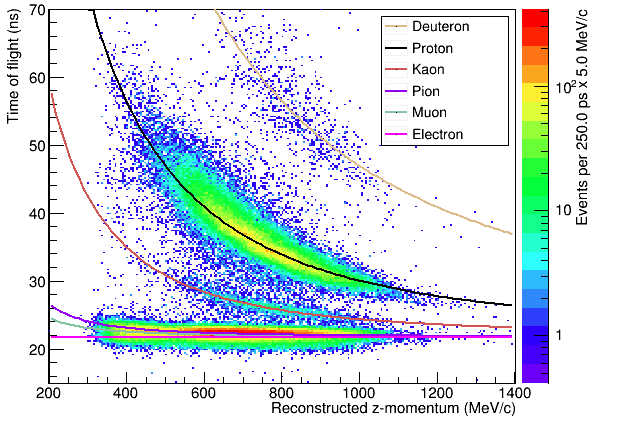
\includegraphics[width=5in]{images/Lariat/KaonTOF}
\caption{Time of flight versus momentum distributions as produced by the LArIAT TOF and Wire Chambers systems. The Kaon population lies between the proton and the muon/pion populations, allowing PID of Kaons in the beam line.  }
\label{fig:TOFK}
\end{figure}

In this energy range, the relevant K-Nucleon interactions are according to \cite{fesbach1992theoretical}:
\begin{equation}
K^{+} + N \rightarrow K^{+} + N\textit{ (elastic)}
\end{equation}
\begin{equation}K^{+} + n \rightarrow K^{0} + p\textit{ (elastic)}\end{equation}
\begin{equation}K^{+} + N \rightarrow K + N + \pi \textit{ (inelastic)}\end{equation}
\begin{equation}K^{+} + N \rightarrow K^{*} + N\textit{ (inelastic)}.\end{equation}



\subsubsection{K$^{+}$Ar Cross section in the Context of Light Mesons Interaction with Nuclei}
\label{sec:theoryStrangeMeson}
The intrinsic value of this measurement is that kaon interactions complement the measurements of $\pi$ interactions as a probe of  hadron interaction inside the nucleus in the strange sector.  
\textcolor{red}{CHIEDI REFERENZE A FLAVIO}

\subsubsection{K$^{+}$Ar Cross section in the Context of Nucleon Decay Searches}
\label{sec:theoryPDK}
Baryon number is accidentally conserved in the Standard Model. Even though no baryon number violation has been experimentally observed thus far, no underlying symmetry in line with the Noether paradigm \cite{Noether1971} explains its conservation. Almost all Grand Unified Theories predict at some level baryon number violation in the form of nucleon decay on long time-scales.  Given the impossibility to reach grand unification energy scales with collider experiments ($\sqrt{s} > 10^{15}$ GeV),  an indirect proof of GUT is needed. The experimental observation of nucleon decay may be the only viable way to explore these theories and it is therefore a subject of great interest \cite{Adams:LBNE}. %Both experiments and theory indeed suggest the energy scale for convergence of the running coupling constants of the Standard Model to be over $10^{15}$ GeV. This energy scale seems impossible to access by any foreseeable accelerator experiment, leaving baryon number violation  to be the only testable process. 

If nucleon decay was experimentally found, additional information about the GUT type may be derived from the dominant decay mode. 
Supersymmetric GUTs \cite{Dimopoulos:1981dw,Bajc20161} prefer the presence of kaons in the products of the decay, e.g. $p\rightarrow K^+\bar{\nu}$  (see fig \ref{fig:MandatoryFeynmannDiagrams}, left).
%%%%%%%%%%%%%%%% Find theory papers!!!!!! %%%%%%%%%%
Gauge mediation GUTs, in which new gauge bosons are introduced that allow for the transformation of quarks into leptons, and vice versa, prefer the mode $p\rightarrow e^+\pi^0$ (see fig \ref{fig:MandatoryFeynmannDiagrams}, right).



\begin{figure}[hbpt]
\centering
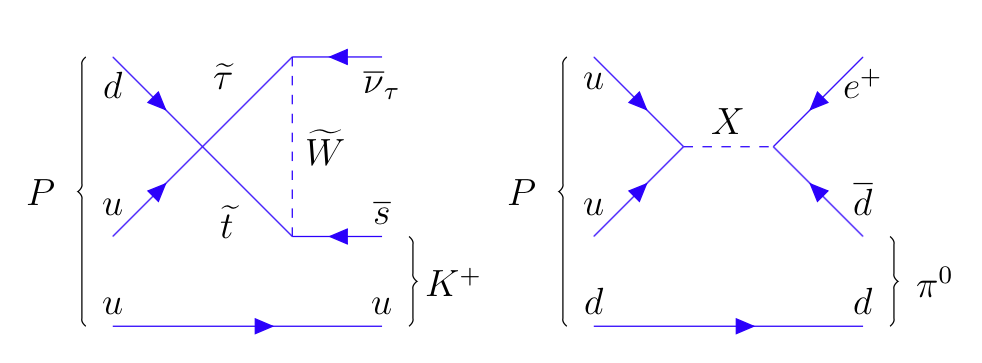
\includegraphics[width=6.5in]{images/MandatoryFeynmannDiagrams.png}
\caption{Feynman diagrams for proton decay ``golden modes": $p \rightarrow K^+ \bar{\nu}$ for supersymmetric GUTs on the left and  $p \rightarrow e^+ \pi^0$ for gauge-mediation GUTs  on the right.}
\label{fig:MandatoryFeynmannDiagrams}
\end{figure}

The key elements for a rare decay experiment are: massive active volume, long exposure, high identification efficiency and low background. 
%The limit to proton lifetime in case of absence of signal and backgrounds is set by calculating
%$$\tau/B > M\times \epsilon\times T \times 10^{32},$$ 
%where M is the detector mass in kton, $\epsilon$ the signal detection efficiency after cuts to suppress backgrounds (dependent on the considered decay mode), T is the exposure in years, B the assumed branching fraction for the considered mode and  $10^{32}$ is a factor accounting for the number of nucleons in a kton of material \cite{Bueno2007}.
Figure \ref{fig:PDKExperimentalLImit} shows the current best experimental limits on nucleon decay lifetime over branching ratio (dots). Historically, the dominant technology used in these searches has been water Cherenkov detectors: all the best experimental limits on every decay mode are indeed set by Super-Kamiokande \cite{PhysRevD.90.072005,PhysRevLett.115.121803}.  It is particularly important to notice that the kaon energy for the proton decay mode $p \rightarrow K^+ \bar{\nu}$ is under Cherenkov threshold.  Super-Kamiokande set the limit on the lifetime for the $p \rightarrow K^+ \bar{\nu}$ mode by  relying exclusively on photons from nuclear de-excitation. For this reason, an attractive alternative approach to identifying nucleon decay is the use of a Liquid Argon Time Projection Chamber (LArTPC). 

LArTPCs can complement nucleon decay searches in modes where water Cherenkov detectors are less sensitive, especially $p\rightarrow K^+\bar{\nu}$.
%The stars in Figure \ref{fig:PDKExperimentalLImit} show the projected sensitivities for new generation of nucleon decay experiments: DUNE (LArTPC) and Hyper-K (water Cherenkov).
According to \cite{Acciarri:Dune}, DUNE will have an active volume large enough, have sufficient shielding from the surface, and will run for lengths of time sufficient to compete with Hyper-K, opening up the opportunity for the discovery of nucleon decay. 

\begin{figure}[hbpt]
\centering
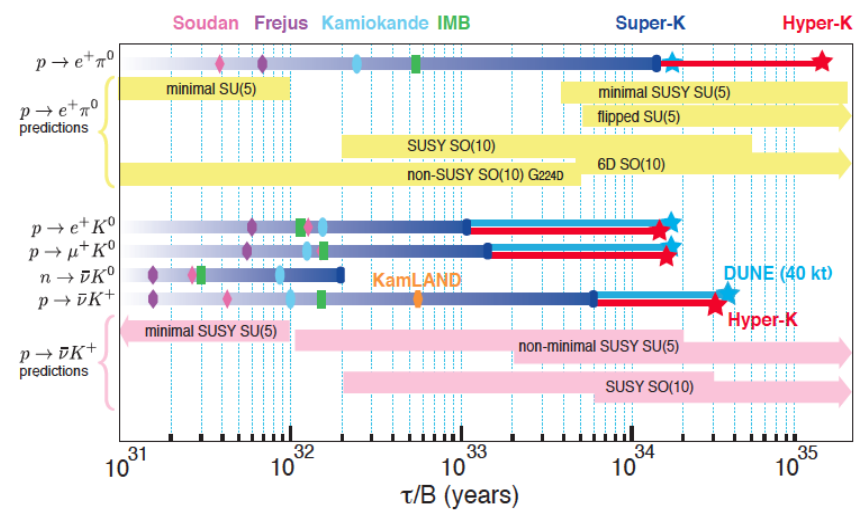
\includegraphics[width=6.5in]{images/PDKExperimentalLImit.png}
\caption{Proton decay lifetime limits from passed and future experiments.}
\label{fig:PDKExperimentalLImit}
\end{figure}

Of course, LArIAT tiny active volume makes it impossible for the experiment to place competitive limits on nucleon decay.  
However,  LArIAT provides excellent data to characterize kaons in LAr for the ``LAr golden mode" $p \rightarrow K^+ \bar{\nu}$. The result of these studies will affect future proton decay searches in LArTPCs. Previous work has been done to assess the potential identification efficiency for different decay modes in a LArTPC \cite{Bueno2007}, but, as the time of this  writing, no study of kaon selection efficiency in LArTPCs has been performed on data. 
The K$^+$-Ar interaction cross section has never been measured before and can affect the possibility of detecting and measuring kaons when produced in a proton decay event. 
Kaon interactions with argon can distort the kaon energy spectrum as well as change the topology of single kaon events. In a LArTPC, non-interacting kaons appear as straight tracks with a high ionization depositions at the end (Bragg peak). The topology of interacting kaons can be quite different. In case of elastic scattering, a distinct kink will be present in the track. In case of inelastic scattering the Bragg peak will not be present and additional tracks (pions) will populate the event.
Performing the total K$^+$-Ar cross section measurement on data serves the double purpose of identifying the rate of ``unusual" topologies (kinks and additional tracks) and of developing tools for kaon tracking in LAr.


\subsection{Previous Measurements: Lighter and Heavier Nuclei}
In general, data on kaon cross sections are  extremely scarce. The measurement of kaon interaction cross section would bring the additional benefit of reducing the uncertainties associated  with hadron interaction models adopted in MC simulations for argon targets.

The data on nuclear effects for specific hadronic final states are extremely scarce, resulting in big uncertainties in modeling final state interactions \cite{Drakoulakos:2004gn}. Figure \ref{fig:Friedmann} shows a 1997 measurement on several elements as performed by  Friedmann et al.  \cite{Friedman:1997eq}. As a reference, this paper measures a $\sigma_{Tot}$ for Si of  366.5  $\pm$  4.8 mb and a $\sigma_{Tot}$ for Ca of 494.6  $\pm$ 7.7 mb at 488 MeV/c.  The cross section for argon is expected to lie in between these two measurements. 
Additional data on the kaon cross section are provided by Bugg et al. \cite{PhysRev.168.1466}. Bugg performs a measurement of the total 
K$^+$ and K$^-$ cross sections on protons and deuterons over the range of 0.6-2.65 GeV/c, as well as a measurement of the total K$^+$ and K$^-$  cross sections on carbon for a number of momenta; the results of this paper on carbon are reported in Figure \ref{fig:Bugg}.




\begin{figure}
\captionsetup{justification=raggedright}  
\begin{minipage}[b]{.5\textwidth}  
  \centering  
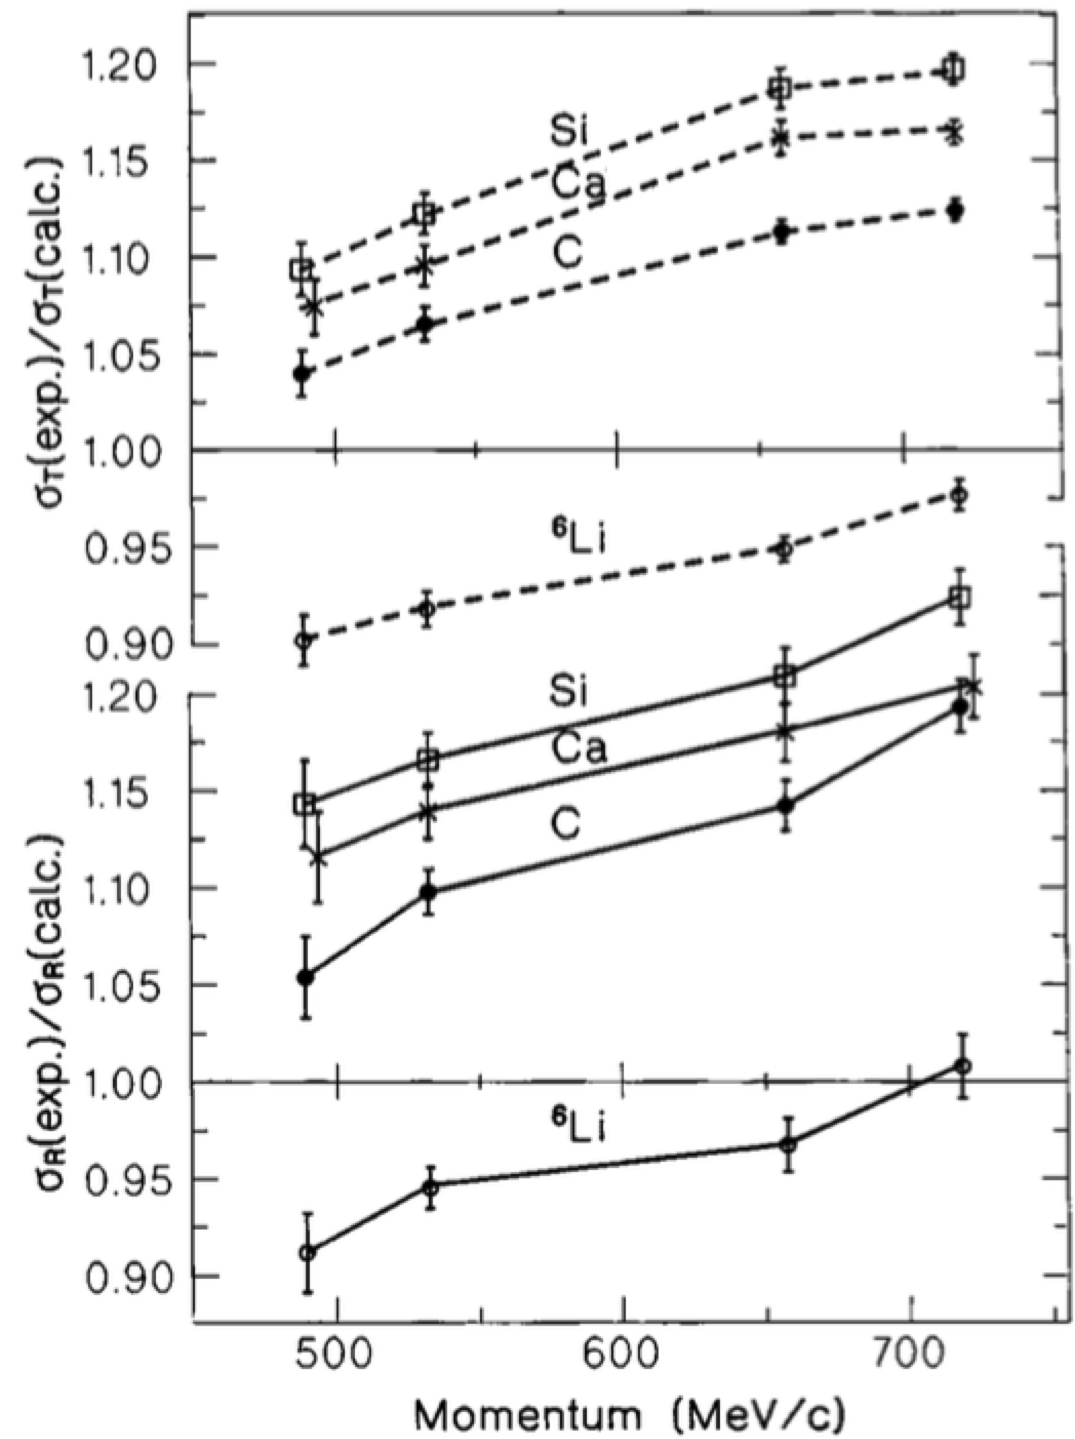
\includegraphics[width=3in]{images/Lariat/Friedmann.png}
\end{minipage}%  
\begin{minipage}[b]{0.5\textwidth}  
  \centering  
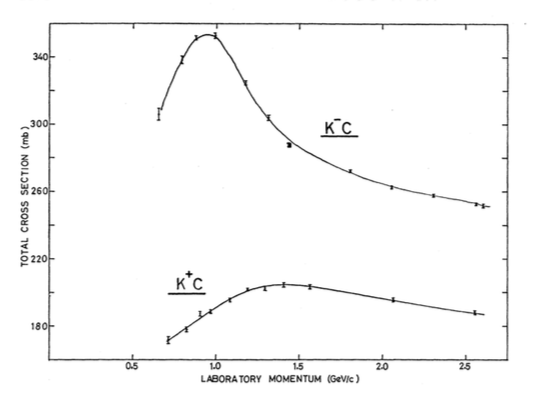
\includegraphics[width=3in]{images/Lariat/Bugg.png}
\end{minipage}
\par
\begin{minipage}[t]{.53\textwidth}
\caption{Ratios between experimental and calculated cross sections as from \cite{Friedman:1997eq}. Top: Total cross sections. Bottom: reaction cross sections.}
\label{fig:Friedmann}
\end{minipage}%
\begin{minipage}[t]{.5\textwidth}  
\caption{Total K$^+$  and K$^-$ cross sections on carbon as from \cite{PhysRev.168.1466}.}
\label{fig:Bugg}
\end{minipage}  
\end{figure}



%%%%%%%%%%%%%%%%%%%%%%%%%%%%%%%%%%%%%%%%%%%%%%%%%%%%%%%
%% PRETTY EVENT DISPLAY WITH TEXT, NOT SURE IF USEFUL
%\begin{figure}[h!]
%\centering
%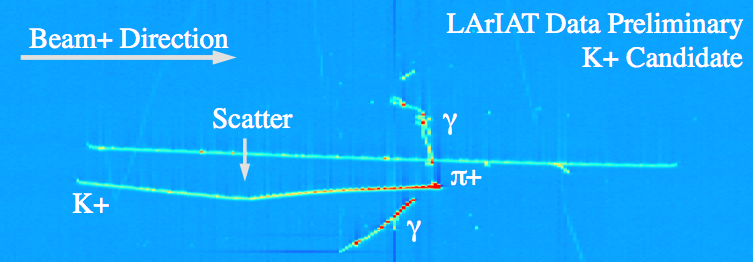
\includegraphics[width=6.5in]{images/Lariat/KLariat.png}
%\caption{LArIAT Data $K^+$ candidate. $K^+$ enters TPC, undergoes a hadronic scatter, and then decays into $\pi^+$ and $\pi^0$. The the $\pi^0$ decays into 2 photons while the $\pi^+$ stops quickly in the TPC. Collection plane view.}
%\label{Fig:KLariat}
%\end{figure}

%Fig \ref{Fig:KLariat} shows a $K^+$ candidate event in the LArIAT TPC. Following the kaon candidate track from left to right, two important elements are visible by eye: a change in the K momentum due to hadronic scatter and a Bragg peak by the end of the track due to an augment of ionization as the kaon slows down in the TPC. The track "kink" is only visible thanks to the millimetric spacial resolution of the TPC, while the Bragg shows the calorimetric power of this technology. The kaon in this event decays hadronically into $\pi^+$ and $\pi^0$. The the $\pi^0$ decays into 2 photons while the $\pi^+$ stops quickly in the TPC. The ability to distinguish the topology of this decay from the most frequent one, i.e. $K^+\rightarrow\mu^+\nu$, remarks the versatility of the LArTPC technology.
%%%%%%%%%%%%%%%%%%%%%%%%%%%%%%%%%%%%%%%%%%%%%%%%%%%%%%%




 \subsection{Kaon Interaction Cross Section for thin target in Geant4}
Since the kaon cross section in argon has never been measured before, the Geant4 Monte Carlo tunes kaon transportation in argon by extrapolation from lighter and heavier nuclei. As shown in the previous section,  kaon data on carbon are available and  can be used as a metric to evaluate the Geant4 prediction performances.  Figure \ref{fig:TrueCarbon} shows the total hadronic cross section for carbon implemented in Geant4 10.01.p3 overlaid with the Bugg and Friedman data. Unfortunately, the current version of Geant4 does not reproduce the data for carbon closely. On one hand, this evidence makes us even more wary when using the Monte Carlo in simulating the kaon-argon interactions. On the other, it further highlights the importance of kaon measurements.

The K$^{+}$Ar cross section implemented in Geant4 can still be used as a tool to validate the measurement methodology. For the considered energy range, the Geant4 inelastic model adopted to is ``BertiniCascade", while the elastic model ``hElasticLHEP".  Figure \ref{fig:TrueArgon} shows the total hadronic cross section for argon implemented in Geant4 10.01.p3 (solid lines) overlaid with the true MC cross section as obtained with the sliced TPC method (markers); the total cross section is shown in green,  the elastic cross section in blue and the inelastic cross section in red. The sliced TPC method described in sec \ref{sec:KXSStrategy}. For the methodology validation we use the true energy deposition for a pool of about 140000 kaons fired inside the LArIAT TPC active volume and a uniform slice length of 4.7 mm.  The nice agreement with the Geant4 distribution and the cross section  obtained with the sliced TPC method gives us confidence in the  validity of the methodology. 
        
     
\begin{figure}
\captionsetup{justification=raggedright}  
\begin{minipage}[b]{.53\textwidth}  
  \centering  
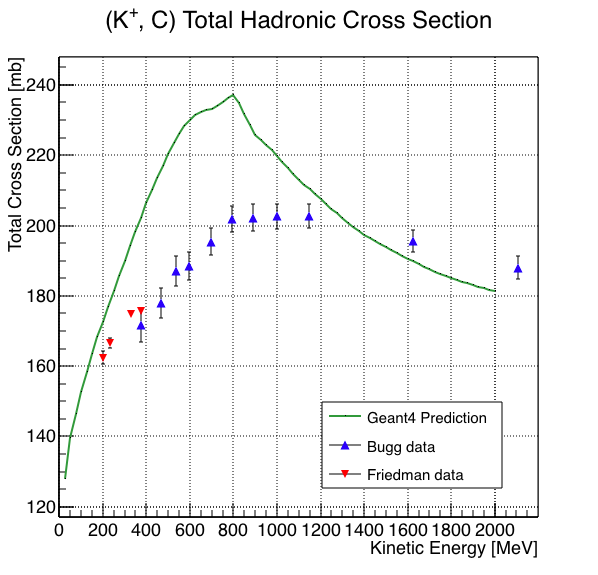
\includegraphics[width=3in]{images/Lariat/CarbonG4.png}
\end{minipage}%  
\begin{minipage}[b]{0.53\textwidth}  
  \centering  
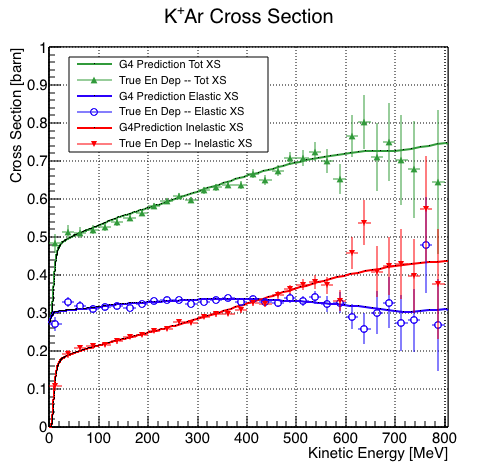
\includegraphics[width=3in]{images/Lariat/KaonTrueXS.png}
\end{minipage}
\par
\begin{minipage}[t]{.53\textwidth}
\caption{total hadronic cross section for carbon implemented in Geant4  10.01.p3  with overlaid with the Bugg and Frideman data.}
\label{fig:TrueCarbon}
\end{minipage}%
\begin{minipage}[t]{.5\textwidth}  
\caption{Hadronic cross sections for argon implemented in Geant4 10.01.p3 (solid lines) overlaid the true MC cross section as obtained with the sliced TPC method (markers). The total cross section is shown in green,  the elastic cross section in blue and the inelastic cross section in red.}
\label{fig:TrueArgon}
\end{minipage}  
\end{figure}






%%%%%%%%%%%%%%%%%%%%%%%%%%%%%%%%%
%% SECTION 2: Data Samples
%%%%%%%%%%%%%%%%%%%%%%%%%%%%%%%%%
\newpage
\section{Analysis strategy}\label{sec:kaonAnalysis} 
 
In this section, we will give an overview of the $K^{+}$-Ar total cross-section analysis strategy. 
The strategy can be summarize in 3 steps:
\begin{itemize}
\item[1.] Identification of kaon candidates in the beam line.
\item[2.] Application of the ``thin-slice'' method.
\item[3.] Identification and treatment of the slices containing a decaying kaon.
\end{itemize}

\subsection{Identification of kaons in the beam line}
First task of this analysis is selecting the kaon candidates in the LArIAT beam line data.

In order to do so,  it is beneficial to describe how LArIAT gets its beam of charge particle to the TPC. A primary beam of 120~GeV protons is transported to the Meson Building and split to make two beam lines known as MCenter and MTest. LArIAT is served by the MCenter beam line, whose primary beam of 120~GeV protons impinges upon a thick target (25~cm) to create a secondary beam of charged particles, mainly pions, in the 8 - 80 GeV range. This collimated pion beam is momentum-selected and then transported the MC7 radiation enclosure, the LArIAT experiment hall.  

In the MC7 enclosure the secondary beam focuses onto a thick copper target and the resulting tertiary beam is collimated by a 1~m iron shield with an opening $-13\deg$ to beam's right with respect to the secondary beam direction. Two analyzing dipole magnets steer the beam path $+10\deg$, selecting a momentum window within 0.2 and 2.0~GeV/c. The polarity of the magnets determines the sign of the selected particles (positive or negative runs). The tertiary beam is instrumented with a pair of Time-of-Flight (TOF) scintillating detectors,  four Wire Chambers (WC), two Aerogel Cherenkov counters (AG), the LArTPC detector and a Muon Range Stack. Figure \ref{fig:beamlineschematic} shows a diagram of the tertiary beam line within the MC7 enclosure.

\begin{figure}[htb]
\begin{center}
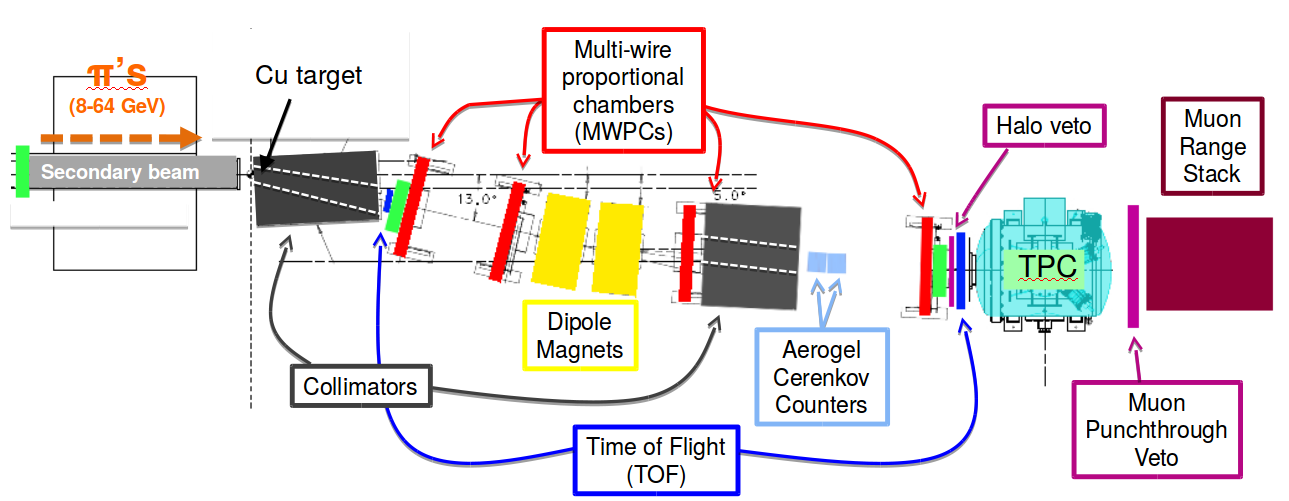
\includegraphics[scale=0.25]{./images/mc7beamline.png}
\end{center}
\caption{Schematic of the Tertiary Beam line within the MC7 enclosure.}
\label{fig:beamlineschematic}
\end{figure}

The beam line kaon candidates are selected by picking out the right events from the tertiary beam line triggered events \textcolor{red}{(Maybe write how triggers are formed?)}.
In this analysis, only the information from the Wire Chambers and the Time-of-Flight is used for particle identification. For the TOF, we use the standard reconstruction software. For the WC, we use the ``picky tracks" reconstruction which requires one and only one hit in all four the wire chambers. From the time of flight and momentum reconstruction, we calculate the mass of a given beam line track using the following equation

\begin{equation}
mass = \frac{p}{c}\sqrt{(\frac{TOF \times c}{l})^2 -1}
\end{equation}
where $p$ represents the measured momentum from the wire chamber, $TOF$ represents the time-of-flight measured as the difference between the two time-of-flight paddles in the LArIAT beam line, $l$ is path length the particle traveled down the beamline, and $c$ represents the speed of light. A selection on the reconstructed mass (350~MeV $<$ mass $<$ 650~MeV) determines the pool of beam line kaon candidates. \\
Once an event is selected in the beam line, we need to match the kaon candidate with a track inside the TPC. 
The last kaon hit recorded in the beam line is at WC4, but WC4 is located 100 cm upstream the TPC front face. In this space the kaon encounters air, the halo veto, the front face of the cryostat and about 10 cm of dead argon. From MC simulation, we estimate that about 26\% of beam line kaon candidates do not reach the TPC: they either interact or decay before the front face. Due to beam line pile up, more than one reconstructed TPC track may be present in the same TPC event. We apply a series of geometrical requirements to match the beam line candidate to a TPC track: we require the position and direction of the TPC track to be consistent with the projection of the WC track at the TPC  front face. If at least one TPC track passes the selection cut, the event is used for the cross section measurement.

\label{sec:BeamlineKStrategy}
\subsection{The thin-slice method}
\label{sec:KXSStrategy}
\subsubsection{Cross Section on Thin Target}\label{sec:thinTargetXS}
Interaction cross sections on thin target are a classic nuclear physics measurement with a well established methodology. A thin target is a target formed by a slab of material containing many uniformly distributed diffusion centers, where  one center is not sitting in front of another.
A pictorial representation of a thin slice experiment is shown schematically in Figure \ref{fig:thinslice}

\begin{figure}[htb]
\centering
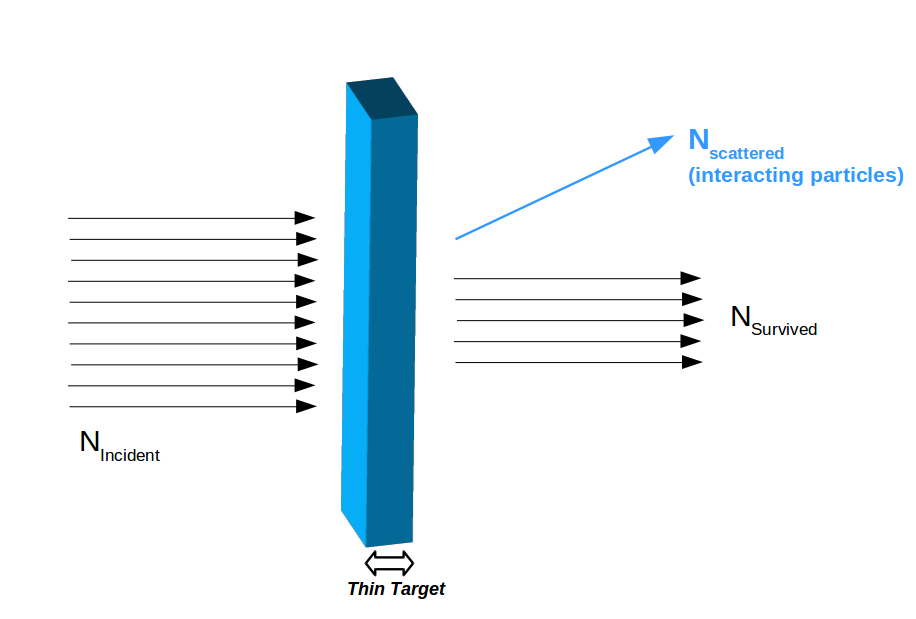
\includegraphics[scale=0.25]{./images/ThinTarget.png}
\caption{Representation of the thin target approximation as a ``thin slice'' of argon experiments.}
\label{fig:thinslice}
\end{figure}

 The survival probability of a kaon traveling through a slab of argon of depth {\it z} and density {\it n} is given by:

\begin{equation}
P_{surv} = e^{-\sigma_{tot}n z}
\end{equation} 
where $\sigma_{tot}$ is the total cross section per nucleon (in $cm^2$), {\textit
{z}} is the target thickness (in cm) along the incident kaon direction, and {\textit
{n}} is the scattering center density in the target, $n=\frac{\rho N_{A} }{A}$ (in $cm^{-3}$). The interaction probability is then $P_{int} = 1 - P_{surv}$. $P_{int}$ is experimentally measured as the ratio of the number of interacting kaons $N_{int}$ over the number of incident kaons $N_{inc}$:
\begin{equation}
P_{int}=\frac{N_{int}}{N_{inc}}=1-e^{-\sigma_{tot}n z}.
\end{equation}

In practices, this assumption of thin target holds true if the target is several order of magnitude smaller than the interaction length. Mathematically speaking, this assumption implies $z\rightarrow\delta z$. Thus, it is possible to Taylor expand the exponential and  solve for the total cross section as a function of energy, $\sigma_{tot}(E)$:
\begin{equation}\label{calc_sigma1}
\frac{N_{int}}{N_{inc}}=1-e^{-\sigma_{tot}n z}\simeq 1-(1-\sigma_{tot}n\delta z + o(\delta z^2)) 
\end{equation}
\begin{equation}\label{calc_sigma2}
\sigma_{tot}(E) \simeq \frac{1}{n\delta z} \Big(\frac{N_{int}}{N_{inc}}\Big) \text{ 	when $z\rightarrow\delta z$}.
%N_{int}(z,E)=(1-N_{inc}e^{-\sigma_{tot}(E)nz})
\end{equation}

In order to measure the cross section, a thin target experiment would simply count the number of incident kaons and the number of surviving kaons.

\subsubsection{Not-so-thin target: sliced TPC}
\label{sec:thick}
The LArIAT TPC, with its 90-cm thick active volume, is not a thin target. Nevertheless, the combination of fine-grained tracking and precise calorimetric information allow us to treat the active volume as a sequence of 240 adjacent thin targets. This technique, called the ``sliced TPC" method, allows to measure the kaon cross section as a function of energy.  In LArIAT, the two wire planes are each made of 240 wires oriented at +/- $60^{\circ}$ with a wire pitch of 4 mm; these planes collect signals proportional to the energy loss of the kaon in a $60^{\circ}$-inclined 4~mm thin slab of liquid argon. Thus, one can think of the TPC as being divided into $\sim$240 slices along the direction of the incident particles ({\textit
{z}} axis) with a spacing $\Delta${\textit
{z}} = 4 mm/sin($60^{\circ}$) $\approx$ 4.5~mm, as shown in Fig.~\ref{fig:slicedtpc}. 
Each slice can be now considered an independent ``thin target" experiment and the cross section calculation in Eq. \ref{calc_sigma2} can be iteratively applied. The kinetic energy of the kaon entering the TPC is determined by measuring its momentum with the tertiary beamline and assuming the kaon mass as mass hypothesis. At each given slice, the kaon incident kinetic  is then determined by subtracting its calorimetric energy released in the previous slice from the total kinetic energy at that slice. Thus, it is possible to perform a differential cross section measurement as a function of the energy because the kaon kinetic energy $K.E._{slice}$  is known before entering each slice. \\ 
When the kaon enters a slice, it contributes to $N_{inc}$ for the energy bin corresponding to  its kinetic energy  that slice. If it interacts in the slice, it also contributes to $N_{int}$ in the appropriate energy bin. If it does not interact, the kaon proceeds to the next slice and the counting is repeated for its new kinetic energy. If a kaon exists the TPC boundaries without interacting (through going event), its track will contribute exclusively to the $N_{inc}$ slices.\\

The uncertainty for each energy bin is calculated by error propagation from the uncertainty on $N_{incident}$ and $N_{interacting}$. 
Since the number of incident pions in each slice is given by a simple counting, it is safe to assume that $N_{incident}$ is distributed as a poissonian with mean and $\sigma^2$ equal to $N_{incident}$ in each bin.  
On the other hand, $N_{interacting}$ follows a binomial distribution: the particle in a given energy bin might or might not interact.  The interaction probability $p$ is $\frac{ N_{interacting}}{N_{incident}}$ and the number of tries $n$ is $N_{incident}$. 
So, the square of the variance for the binomial is given by  $$\sigma^2 = np(1-p) =  N_{incident}\frac{ N_{interacting}}{N_{incident}} (1-\frac{ N_{interacting}}{N_{incident}}) = N_{interacting}(1-\frac{ N_{interacting}}{N_{incident}}).$$

$N_{incident}$ and $N_{interacting}$ are not independent.
The uncertainty on the cross section is thus calculated as 
\begin{equation}
\delta\sigma_{tot}(E) = \sigma_{tot}(E) \Big(\frac{\delta N_{interacting}}{N_{interacting}}+\frac{\delta N_{incident}}{N_{incident}}\Big) 
\end{equation}
where:
\begin{eqnarray}
\delta N_{incident} = \sqrt[]{N_{incident}} \\
\delta N_{interacting} = \sqrt[]{N_{interacting}(1-\frac{ N_{interacting}}{N_{incident}})}.
\end{eqnarray}

%\textcolor{blue}{Sketch of sliced tpc technique?}
\begin{figure}[htpb]
\centering
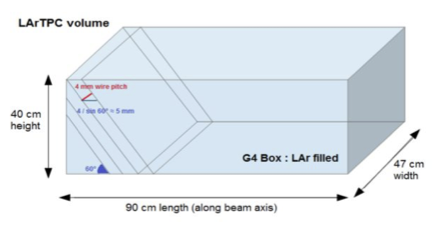
\includegraphics[scale=1.25]{images/Lariat/SlicedTPC.png}\\
\caption{Sketch of Sliced TPC approach.}
\label{fig:slicedtpc}
\end{figure}

It is worth noticing an important difference between the procedure utilized by LArIAT to measure the total hadronic kaon cross section and the procedure used by other experiments in neutrino cross section measurements. In the latter, one needs to correct for the detector inefficiency in identifying neutrinos. In our measurement,  we need do not need to efficiency correct for the beam line candidates which we are not able to identify in the TPC. This is because the cross section calculation in Eq. \ref{calc_sigma2}  relies on measuring the ratio $\frac{ N_{interacting}}{N_{incident}}$, where both these numbers are drawn from tracked kaons in the TPC.

The sliced TPC technique was tested by comparing the results of this method with the Geant 4.10.1.p3 prediction of the total hadronic interaction cross section ($K^{+}$, Ar)  with Bertini Cascade model.
Fig.~\ref{fig:TrueArgon} shows the resulting total ${K^+}$ cross section extracted by the sliced TPC technique; it agrees well with the Geant 4  cross section.  This comparison demonstrates the power of the sliced TPC method for the measurement of the ($K^{+}$, Ar) cross section in LArIAT TPC geometry. 



\subsection{Slices containing decays}
We address here an important difference between the thin target and the thick target experiments. While the fraction of kaon decay in the thin target is negligible, both in flight and at rest decays play an important role in the thick target case. 
Kaon decay proceeds by the weak interaction; since our goal is to measure the hadronic cross section, slices containing decaying kaons must not contribute to the number of interacting slices. If one only considers the endpoint of the primary kaon track without identification of the decay, this slice will  wrongly contribute to the $N_{interacting}$ counting. 

Figure \ref{fig:interactionBreakdown} shows the interaction types as a function of the kaon kinetic energy as predicted by  Geant 4.10.1.p3. The plot is normalized by the total number of simulated events which enter the TPC.
As shown in the figure, kaon decay mainly at rest: about 68\% of decaying kaons has a kinetic energy of less than 50 MeV. 
Figure \ref{fig:interactionBreakdownPercentage} shows the proportional contribution of each interaction type as a function of the kinetic energy as predicted by  Geant 4.10.1.p3. Each bin is normalized by the number of interactions for that kinetic energy.
Given the prominence of decay in the first kinetic energy bin, a simple way to eliminate the contribution from slices containing kaon decay at rest is setting a proper lower bound for the kinetic energy range in the cross section measurement. We decide to measure the cross section in the region between 100 MeV to 1000 MeV \textcolor{red}{(true for now...)}.
Kaon decay in flight are more tricky, since they can happen at any energy. According to Geant4, they make up less than 20\% interactions for energies greater than 100 MeV. A distinction between interaction and decay based on the event topology is thus needed and will be discussed later in the note  \textcolor{red}{(reference to right chapter)}. If a decay is tagged in a slice, the corresponding kinetic energy will contribute exclusively to the $N_{inc}$ counting.\\


%A Bragg peak towards the end of the kaon track is also formed as the kaon comes to a stop. 
     
\begin{figure}
\captionsetup{justification=raggedright}  
\begin{minipage}[b]{.53\textwidth}  
  \centering  
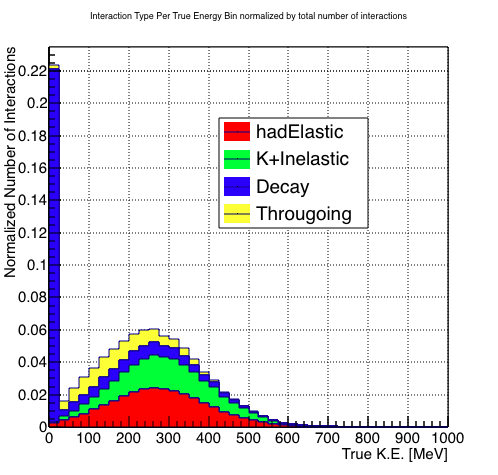
\includegraphics[scale=0.45]{./images/Lariat/InteractionBreakDown.png}
\end{minipage}%  
\begin{minipage}[b]{0.53\textwidth}  
  \centering  
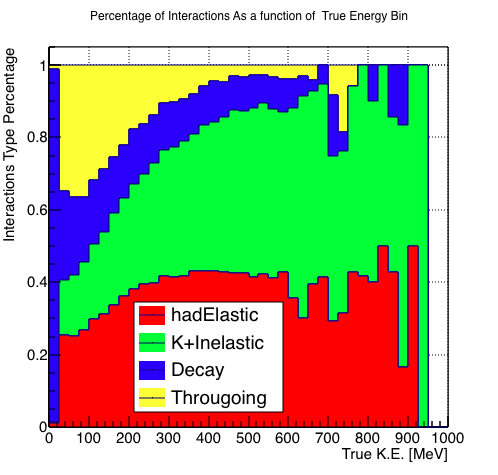
\includegraphics[scale=0.45]{./images/Lariat/PercentageIntType.png}
\end{minipage}
\par
\begin{minipage}[t]{.53\textwidth}
\caption{Interaction types as a function of the kaon kinetic energy as predicted by  Geant 4.10.1.p3: decay (blue), through going (yellow), elastic (red), inelastic (green).}
\label{fig:interactionBreakdown}
\end{minipage}%
\begin{minipage}[t]{.5\textwidth}  
\caption{Proportional contribution of the various interaction types as a function of the kaon kinetic energy as predicted by  Geant 4.10.1.p3: decay (blue), through going (yellow), elastic (red), inelastic (green). Each bin is normalized by the number of interactions for that kinetic energy.}
\label{fig:interactionBreakdownPercentage}
\end{minipage}  
\end{figure}









\newpage
\section{Data / MC Samples}\label{sec:DataSamples}

This section outlines the data and Monte Carlo sets used in this analysis. \\
For the data, we are using a set which spans all of Run-II positive polarity data. Details on this sample can be found in Section \ref{sec:data}. For the simulation, we use the G4Beamline Monte Carlo (Section \ref{sec:G4Beamline}) and the Data Driven single particle Monte Carlo (DDMC, Section \ref{sec:DDMCSamples}). 


%%%%%%%%%%%%%%%%%%%%%%%%%%%%%%%%%%%%%%%%%%%%%%
\subsection{Data}\label{sec:data}
%%%%%%%%%%%%%%%%%%%%%%%%%%%%%%%%%%%%%%%%%%%%%%



LArIAT successfully ran for 9 weeks in 2015 (Run I) and 24 weeks in 2016 (Run II). Some spectacular kaon interactions were found in data from Run I (see Figure \ref{fig:MCdata} and its great agreement with the MC),
but the kaon statistics in Run I is not enough to perform a cross section analysis. Figure \ref{fig:BeamComp} shows the reason behind the low statistics: this figure represents the tertiary beam composition of one of the first data runs. Two aspects of this plot are particularly notable. Firstly, kaons are very few in the beam. However, the few kaons produced are in the correct range of momentum for proton decay studies (compare the momentum on Figure \ref{fig:KGenie}).  LArIAT Run II provides enough statistic to measure kaon cross section. 
\begin{figure}[hpbt]
\centering
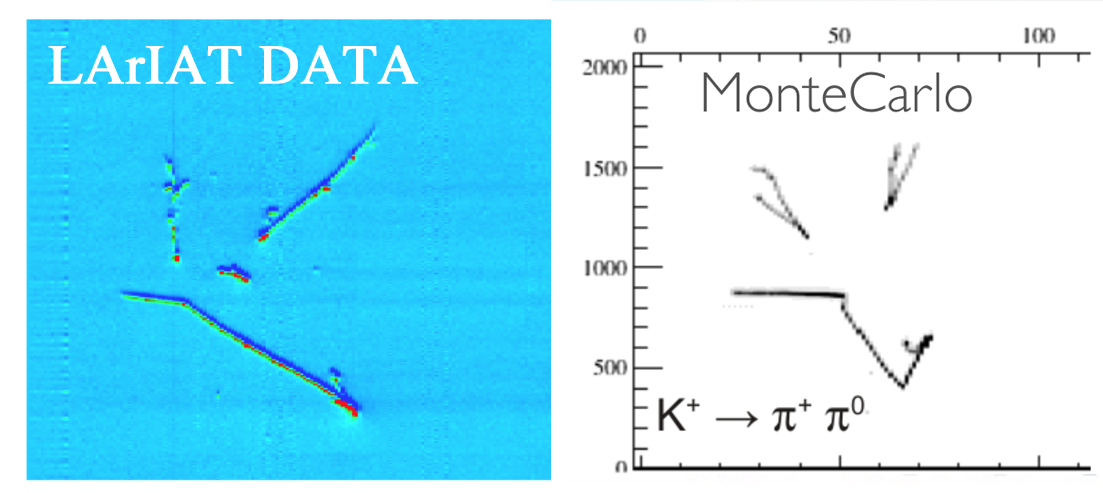
\includegraphics[width=6in]{images/Lariat/KDataMC}
\caption{Direct comparson between a kaon event in LArIAT Run I data and in LArIAT MC. }
\label{fig:MCdata}
\end{figure}


\begin{figure}[h!]
\centering
\begin{minipage}{0.45\textwidth}
\centering
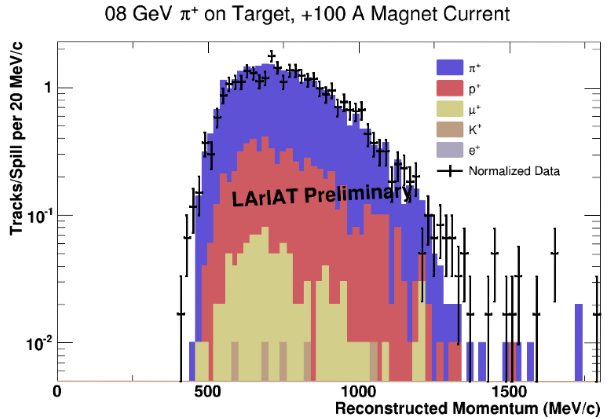
\includegraphics[width=3.5in]{images/Lariat/Beam}
\caption{Particle spectrum at the TPC produced with the LArIAT 8 GeV tertiary beam.}
\label{fig:BeamComp}
\end{minipage}\hfill
\centering
\begin{minipage}{0.45\textwidth}
\centering
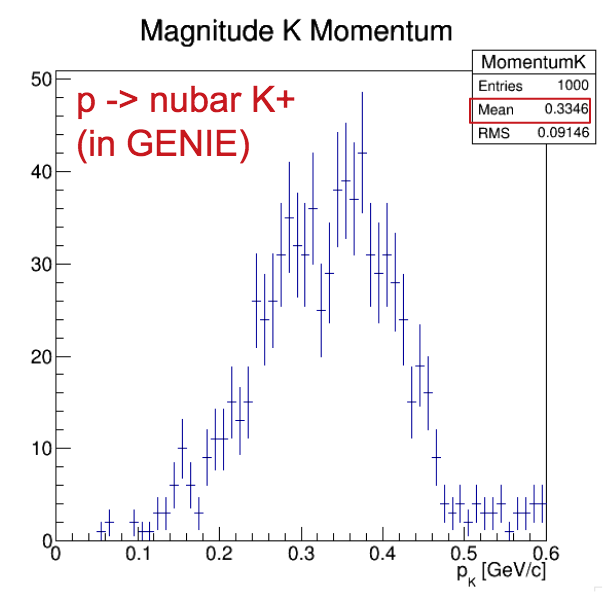
\includegraphics[width=3in]{images/Lariat/KaonGenie}
\caption{Momentum distribution for the kaon in the $p \rightarrow K^{+} \bar\nu$ mode proton decay as simulated by GENIE.}
\label{fig:KGenie}
\end{minipage}
\end{figure}





\begin{center}
\begin{table}[b]
	\begin{center}
	%\resizebox{0.95\textwidth}{!}{%
	\begin{tabular}{|c|c|c|}
	\multicolumn{3}{c}{\textbf{Summary of Data Samples}} \\
	\hline \hline
	 Run Period & Data Set Definition & Samweb Meaning \\
%	\hline
%	 &  & \verb!defname: TPC_voltages_nominal! \\
%	\hline
%	 &  & \verb!TPC_MaxGainAndFilter! \\
%	\hline
%	Run-I & \verb!Lovely1_Neg_RunI_elenag_v02! & \verb!TPC_nominal_read_out_and_timing!  \\
%	\hline
%	 & & \verb!BothTOF_OnAndReadOut!  \\
%	\hline
%	 & & \verb!AllMWPC_OnAndReadOut!  \\
%	 \hline
%	 & & \verb!lariat_mid_f_mc7anb < 0! \\
%	\hline
%	\line
%	 & & \verb!run_number >= 8000 and run_number <= 10226! \\
     \hline	
	&  & \verb!defname: TPC_voltages_nominal! \\
	\hline
	 &  & \verb!TPC_MaxGainAndFilter! \\
	\hline
	Run-II & \verb!Lovely1_Pos_RunII_elenag_v04! & \verb!TPC_nominal_read_out_and_timing!  \\
	\hline
	 & & \verb!BothTOF_OnAndReadOut!  \\
	\hline
	 & & \verb!AllMWPC_OnAndReadOut!  \\
	 \hline
	 & & \verb!lariat_mid_f_mc7anb > 0! \\
	 	 \hline
	 & & \verb!create_date < '2017-06-02'! \\

	 \hline
	\end{tabular}%}
	\caption{Summary of the data sample used for this analysis. }
	\label{tab:datasamples}
	\end{center}
\end{table}
\end{center}

The Run-II data use the definitions \href{https://redmine.fnal.gov/redmine/projects/lardbt/wiki/Recommended_SAM_Datasets}{oulined on this Wiki page} and summarized in Table \ref{tab:datasamples}.


The relevant \texttt{samweb} definitions listed in Table \ref{tab:datasamples} which require some explaining are defined as:

\begin{itemize}
\item \textbf{TPC Voltages Nominal}: Requires the cathode to be at greater than 23 kV, the collection plane wires voltage to be between 320 and 350 V, the induction plane voltage to be between -10 and -20 V, and the shield plane voltage to be greater than -310 V

\item \textbf{TPC MaxGainAndFilter}: Requires the ASIC configuration to be set as ``3'' for both the filter and the gain setting

\item \textbf{TPC Nominal Read Out and Timing}: Requires the readout of the TPC was enabled, the recorded number of time ticks is 3072, and the delay of 36900 was set on the v1495 (trigger card).
\item \textbf{lariat\_mid\_f\_mc7anb \textgreater 0} : Requires the polarity of the magnets to be positive
\item \textbf{create\_date \textless  2017-06-02}: Avoids the introduction of run 3 data and newly sliced data
\end{itemize}


It is important to provide a break down of the beam conditions for the period of data taking because the beam composition, hence the kaon content, varies according to the energy of the secondary beam and the strength of the magnetic field. Table \ref{tab:beamConditions} shows a break down of the beam conditions for the beam data selected by  \verb!Lovely1_Pos_RunII_elenag_v04! and the events that pass the beam line  selection.


\begin{table}[]
\centering
\caption{Break down of beam conditions for Run-II positive polarity data. $I$ is the value of the current in the magnets and $E$ is the energy of the secondary beam.  }
\label{tab:beamConditions}
\begin{tabular}{l|l|l|l|l|}
\cline{2-5}
                                       & \multicolumn{2}{l|}{Lovely1\_Pos\_RunII\_elenag\_v04} & \multicolumn{2}{l|}{Beamline Kaon candidate sample} \\ \cline{2-5} 
                                       & Run \% & Event \% & Run \% & Event \% \\ \hline
\multicolumn{1}{|l|}{I = + 100 A, E = 64 GeV}   &   61.8          &        75.0   & 75.1  &  90.35   \\ \hline
\multicolumn{1}{|l|}{I =   + 60 A, E = 64 GeV}   &    30.1         &         23.8  & 24.9  &   9.65     \\ \hline
\multicolumn{1}{|l|}{Info not available}              &      8.1         &           1.2   &    0.0 &       0.0               \\ \hline
\end{tabular}
\end{table}



%%%%%%%%%%%%%%%%%%%%%%%%%%%%%%%%%%%%%%%%%%%%%%%%%%%%%%%%%%%%
\subsection{Monte Carlo Samples}\label{sec:MCSamples}
For the simulation of the tertiary beam, we use a combination of two MC generators: the G4Beamline Monte Carlo and the Data Driven single particle Monte Carlo (DDMC).   We use the G4Beamline MC to calculate the particle composition of the beam just before the cryostat. In order to simulate the beam line particles after Wire-Chamber 4, we use the DDMC. 

\subsubsection{G4Beamline }\label{sec:G4Beamline}
At the moment of this writing,  G4Beamline simulates transportation of particles through the beam line from the LArIAT target until ``Big Disk'', a fictional, void detector located just before the cryostat. The responses of  the beam line detectors are not simulated. 

The two beam conditions relevant for this analysis are simulated: secondary beam energy of 64 GeV, positive polarity magnet with current of 100 A and 60 A. Figure \ref{fig:beamspectrum} shows the tertiary beam spectra for the 64 GeV and 100 A condition on the left and for the 64 GeV and 60 A condition on the right.
In Table \ref{tab:beamcomp2}, the beam composition is given in terms of percentage of different particle species per spill for positive polarity. The values reported are the weighted average on the two beam conditions considered. The weights are calculated according to the fourth column of Table \ref{tab:beamConditions}. 

\begin{table}[ht!]
\centering
\begin{tabular}{|l|l|l|l|l|l|l|}
\hline
                   & $\pi^+$ & $e^+$ & $\gamma$ & $\mu^+$ & $K^+$ & p \\ \hline
Beam Composition (\%) &    42.8     &  30.1     &    8.6      &    2.1     &    0.057    &    16.2            \\ \hline
\end{tabular}
\caption{Beam Composition - Positive polarity configuration (from MC)}
\label{tab:beamcomp2}
\end{table}



\begin{figure}[htb]
\begin{center}

\includegraphics[scale=0.05]{images/dummy.png}
\end{center}
\caption{G4Beamline tertiary beam  predicted spectra for positive 100 Amp, 64 GeV target energy with data overlaid (left). G4Beamline tertiary beam  predicted spectra for positive 60 Amp, 64 GeV target energy with data overlaid (right).}
\label{fig:beamspectrum}
\end{figure}



\subsubsection{Data Driven Single Particle MC (DDMC) }\label{sec:DDMCSamples}
%%%%%%%%%%%%%%%%%%%%%%%%%%%%%%%%%%%%%%%%%%%%%%%%%%%%%%%%%%%%
The DDMC uses the data momentum and position at wire chamber 4 to derive its initial conditions. The details of these samples and where they can be found are given in \href{https://docs.google.com/spreadsheets/d/1_0kNCKBIIx53f6vopqN2OijtcTICHD9rDvN_YKGH2mI/edit?usp=sharing}{this data production spreadsheet}.
More details of how the Monte Carlo used is generated are given in \href{https://lartpc-docdb.fnal.gov:441/cgi-bin/ShowDocument?docid=2054}{docDB-2054} and  \href{https://lartpc-docdb.fnal.gov:441/cgi-bin/ShowDocument?docid=2056}{dobDB-2056}, a summary of which is presented here. 

The Data Driven Monte Carlo (DDMC) uses data quantities for a sample of Wire-Chamber tracks to derive the momentum ($P_x, P_y, P_z$) and position at WC4 $X, Y$ distributions that are seen during a particular running period and/or running condition. Using those data derived distributions, it then launches single particle MC from $z = -100$~cm (the location of the fourth wire chamber) with these distributions as a template. An illustration of this procedure is shown in Figure \ref{fig:DDMC} with the results of the DDMC generation compared to a sample of wire chamber track data. Using this technique ensures the MC and data have very similar momentum, position and angular distributions at Wire-Chamber 4 and allow us to calibrate the energy loss upstream of the TPC as precisely as possible. The DDMC is a single particle Monte Carlo: the beam pile-up is not simulated.

\begin{figure}[htb]
\centering
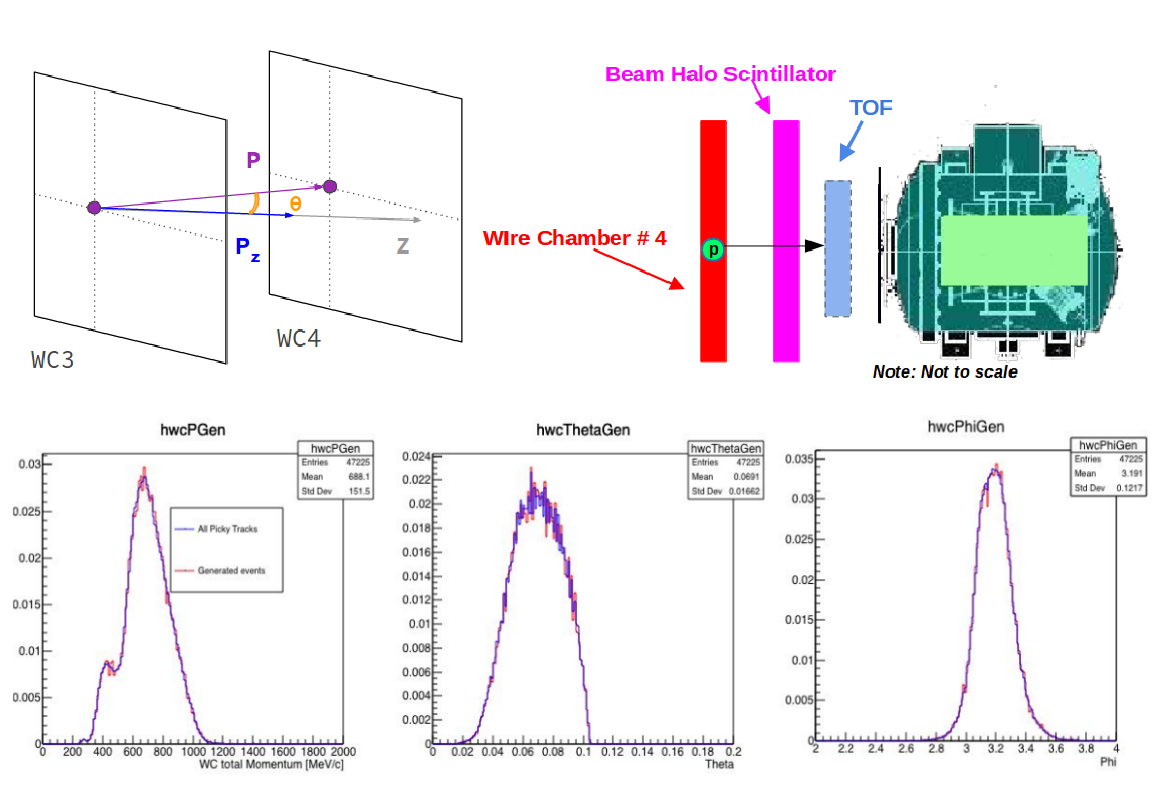
\includegraphics[width=0.70\textwidth]{images/DDMC.png}
\caption{Illustration of the technique where the wire chamber track initial angular and momentum distributions are used to generate the single particle MC.}
\label{fig:DDMC}
\end{figure}

Table \ref{tab:MCSampleGen} lists the various MC samples that were generated for this analysis. 

\begin{table}[htb]
	\begin{center}
	\resizebox{0.95\textwidth}{!}{%
	\begin{tabular}{|c|c|c|}
	\hline
	  \textbf{DDMC Sample} & Original Data Distribution & Number of Events Generated  \\
	  	\hline
	Run-II $\pi^{+}$ & $\pi, \mu, e$ Mass Filter / Picky WC-Track & \\
	Run-II $\mu^{+}$ & $\pi, \mu, e$ Mass Filter / Picky WC-Track &  \\
	Run-II $e^{+}$ & $\pi, \mu, e$ Mass Filter / Picky WC-Track & \\
	Run-II $K^{+}$ & $K^{+}$ Mass Filter / Picky WC-Track & \\
	Run-II $p$ & $p$ Mass Filter / Picky WC-Track & \\
	\hline
	\end{tabular}}
	\caption{Summary of MC generated for the analysis.} \label{tab:MCSampleGen}
	\end{center}
\end{table}

\textcolor{red}{CHECK WITH THE BEAMLINE MC IF WE REALLY NEED THIS}
In addition to this sample of DDMC, a sample of photons is also generated since as is shown in Table \ref{tab:beamcomp1} a small but non-negligible portion of the beam will have photons entering the TPC. This sample is generated with a flat momentum spectrum between 0 MeV and 2000 MeV with a Gaussian angular distribution of $\pm$5 degrees about the beam direction. The photon momentum spectrum is then re-weighted by the momentum spectrum of the corresponding run period it is being simulated for. This approximation allows us to estimate the contamination due to photons from MC with a reasonable assumption of their spectrum.



\newpage

%%%%%%%%%%%%%%%%%%%%%%%%%%%%%%%%%%%%%%%%%%%%%%%%%%%%%%%%%
\section{Kaon candidate selection in the beamline}\label{sec:BeamlineSelection}
\subsection{Overview of the LArIAT Beamline}\label{sec:BeamlineOverview}
%%%%%%%%%%%%%%%%%%%%%%%%%%%%%%%%%%%%%%%%%%%%%%%%%%%%%%%%%

%%%%%%%%%%%%%%%%%%%%%%%%%%%%%%%%%%%%%%%%%%%%%%%%%%%%%%%%%%%%%%%%%%%%%%%%%
\subsection{Beam composition}\label{sec:G4BeamlineMC}
%%%%%%%%%%%%%%%%%%%%%%%%%%%%%%%%%%%%%%%%%%%%%%%%%%%%%%%%%%%%%%%%%%%%%%%%%



\subsection{Data Selection Cut}\label{sec:DataSelectionCut}
\subsubsection{Beamline Candidates}\label{sec:BeamlineCandidates}

%%%%%%%%%%%%%%%%%%%%%%%%%%%%%%%%%%%%%%%%%%%%%%%%%%%%%%%%%%%%
For each sample listed in Table \ref{tab:datasamples}, we outline the event selection used to select this data.

\begin{itemize}
\item \textbf{Time Stamp Filter}

A filter is used to select events which occurred in time with the beam. These events typically coincide with the first 6 seconds of the beam spill, and therefore the events are filtered using the following LArIATsoft settings

\begin{verbatim}
tfilt:      @local::lariat_timestampfilter

# ====================================================================
# Specify range of events to select.  For Run I/II:
#   - pedestal events:  ~ 0.  - 1.2 sec
#   - beam events:      ~ 1.2 - 5.5 sec
#   - cosmic events:    ~ > 5.5 sec
#   (default selects ALL events)
physics.filters.tfilt.T1:                       1.2
physics.filters.tfilt.T2:                       5.5
physics.filters.tfilt.RequireRawDigits:         true

\end{verbatim}



\item \textbf{Beamline Reconstruction}

The standard LArIAT beamline reconstruction is used to select events which have a wire chamber track and TOF information in an individual event using the following modules.
\begin{verbatim}
### beamline elements ###

wctrack:     @local::lariat_wctrackbuilder
tof:         @local::lariat_tof
agcounter:   @local::lariat_aerogel
\end{verbatim}


\textbf{For Run-I we use these default parameters:}
\begin{verbatim} 
physics.producers.wctrack.PickyTracks:                          false
physics.producers.tof.HitThreshold:                           -10.0  
physics.producers.tof.HitDiffMeanUS:                            0.6  
physics.producers.tof.HitDiffMeanDS:                            1.0  
physics.producers.tof.HitMatchThresholdUS:                      3.0  
physics.producers.tof.HitMatchThresholdDS:                      6.0  
physics.producers.tof.HitWait:                                  20.
\end{verbatim}

\textbf{For Run-II we use these default parameters:}
\begin{verbatim} 
physics.producers.wctrack.PickyTracks:                          false
physics.producers.tof.HitThreshold:                             -3.
physics.producers.tof.HitDiffMeanUS:                            0.5  
physics.producers.tof.HitDiffMeanDS:                            0.4  
physics.producers.tof.HitMatchThresholdUS:                      3.0  
physics.producers.tof.HitMatchThresholdDS:                      6.0  
physics.producers.tof.HitWait:                                  20.
\end{verbatim}

We require the tracks reconstructed in the wire chamber satisfy the criteria known as a ``picky track''. ``Picky tracks'' correspond to tracks reconstructed using hits in all four wire chambers. In these events, one and only one hit in each wire chamber track can be reconstructed per event and the track satisfies a straightness requirement in the Y-Z plane. These tracks have more accurate measure of the particle momentum than the ``high yield'' (HY) tracks.  HY tracks only require hits in three out of four of the wire chamber tracks and can have multiple wire chamber hits reconstructed per event. HY tracks yield better statistics: a subset of HY tracks can be used as a orthogonal sample for the study of systematics. Details about wire chamber track reconstruction can be found in \cite{WCTrackReco}

\item \textbf{Particle Mass Filtering}
Using the beamline reconstruction, it is possible to calculate the mass of a given track, as shown in Figure \ref{fig:mass}. The classification of events into the different samples follows:

\begin{itemize}
\item \underline{$\pi, \mu, e$:} 0~MeV $<$ mass $<$ 350~MeV

\item \underline{kaon:} 350~MeV $<$ mass $<$ 650~MeV

\item \underline{proton:} 650~MeV $<$ mass $<$ 3000~MeV

\end{itemize}

\begin{figure}[htb]
\centering
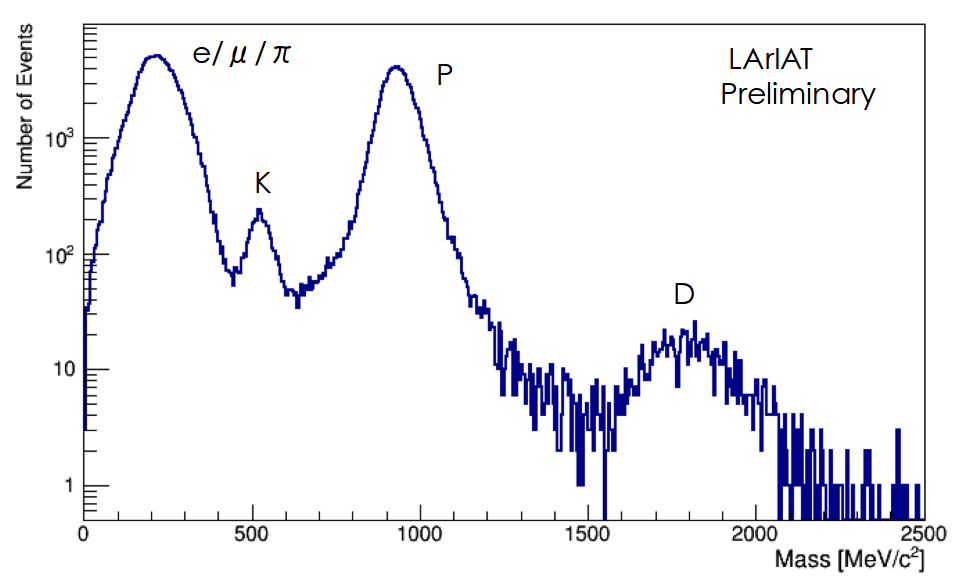
\includegraphics[width=0.70\textwidth]{images/mass.png}
\caption{The mass plotted for a sample of Run-II events reconstructed in the beamline. The classification of the events into $\pi, \mu, e$, kaon, or proton is based on this distribution.}
\label{fig:mass}
\end{figure}

For this analysis we require 350~MeV $<$ mass $<$ 650~MeV to select a sample of $K$ candidates for further event selection. The full event reduction table for these cuts is presented in Section \ref{sec:Results}.

\end{itemize}


\subsubsection{Candidates}\label{sec:Candidates}
\subsubsection{Contamination from different particle species in the beam line }\label{sec:Contamination}
\section{TPC Candidates} \label{sec:TPC} 
\section{Systematics} \label{sec:Systematics} 
\section{Results}\label{sec:Results}

\newpage
%\section{Analysis method}
\subsection{Measurement Strategy -- TPC "slicing"}
\label{sec:KXSStrategy}
A thin target is a target formed by a slab of material containing many uniformly distributed diffusion centers, where  one center is not sitting in front of another. In this approximation, the survival probability of a kaon traveling through a slab of argon of depth {\it z} and density {\it n} is given by:

\begin{equation}
P_{surv} = e^{-\sigma_{tot}n z}
\end{equation} 
where $\sigma_{tot}$ is the total cross section per nucleon (in $cm^2$), {\emph{z}} is the target thickness (in cm) along the incident kaon direction, and {\emph{n}} is the scattering center density in the target, $n=\frac{\rho N_{A} }{A}$ (in $cm^{-3}$). Thus, the interaction probability is $P_{int} = 1 - P_{surv}$. $P_{int}$ is experimentally measured as the ratio of the number of interacting kaons $N_{int}$ over the number of incident kaons $N_{inc}$:
\begin{equation}
P_{int}=\frac{N_{int}}{N_{inc}}=1-e^{-\sigma_{tot}n z}.
\end{equation}

The assumption of thin target implies $z\rightarrow\delta z$. Thus, it is possible to Taylor expand the exponential and  solve for the total cross section as a function of energy, $\sigma_{tot}(E)$:
\begin{equation}\label{calc_sigma1}
\frac{N_{int}}{N_{inc}}=1-e^{-\sigma_{tot}n z}\simeq 1-(1-\sigma_{tot}n\delta z + o(\delta z^2)) 
\end{equation}
\begin{equation}\label{calc_sigma}
\sigma_{tot}(E) \simeq \frac{1}{n\delta z} \Big(\frac{N_{int}}{N_{inc}}\Big) \text{ 	when $z\rightarrow\delta z$}.
%N_{int}(z,E)=(1-N_{inc}e^{-\sigma_{tot}(E)nz})
\end{equation}


LArIAT, with its 90-cm thick active volume, is not a thin target. Nevertheless, the combination of fine-grained tracking and precise calorimetric information allow us to treat the active volume as a sequence of 240 adjacent thin targets. This technique, called the "sliced TPC" method, allows to measure the kaon cross section as a function of energy.  In LArIAT, the two wire planes are each made of 240 wires oriented at +/- $60^{\circ}$ with a wire pitch of 4 mm; these planes collect signals proportional to the energy loss of the kaon in a $60^{\circ}$-inclined 4~mm thin slab of liquid argon. One can thus think of the TPC as being divided into $\sim$240 slices along the direction of the incident particles ({\emph{z}} axis) with a spacing $\Delta${\emph{z}} = 4 mm/sin($60^{\circ}$) $\approx$ 4.5~mm, as shown in Fig.~\ref{fig:slicedtpc}. Each slice can be now considered a "thin target" and the cross section calculation in Eq.~\ref{calc_sigma} can be iteratively applied. It is possible to perform a differential cross section measurement as a function of the energy because the kaon kinetic energy $K.E._{slice}$  at the beginning of slice is known per each slice. The kaon kinetic energy entering the TPC is determined by measuring the particle momentum with the tertiary beamline and assuming the kaon mass as mass hypothesis. At each slice, the incident energy of the kaon is determined by subtraction of the calorimetric energy released by the particle in the previous slice.\\ 
When the particle enters a slice, it contributes to $N_{inc}$ in the energy bin corresponding to its kinetic energy in that slice. If it interacts in the slice, it also contributes to $N_{int}$ in the appropriate energy bin.\\

An important difference between the thin target approximation and the thick target case needs to be address. While in the first case, only the K-nucleus hadronic interactions are taken into account, other processes such as kaon decay, both in flight and at rest play an important role in the "thick" target case. Kaon decays are a physical background for this measurement. Kaon decay proceeds by the weak interaction; if one only considers the endpoint of the primary kaon track without identification of the decay, this process can be misidentified as a single strong interaction. Kaon decay tagging is discussed the next section. 


%\textcolor{blue}{Sketch of sliced tpc technique?}
\begin{figure}[htpb]
\centering
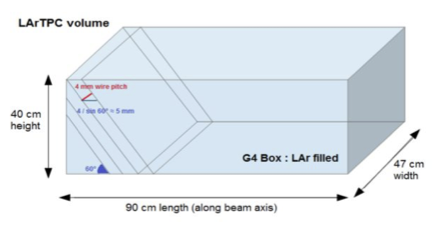
\includegraphics[scale=1.25]{images/Lariat/SlicedTPC.png}\\
\caption{Sketch of Sliced TPC approach.}
\label{fig:slicedtpc}
\end{figure}



%%%%%%%%%%%%%%%%%%%%%%%%%%%%%%%%%
%% SECTION 3:Data Samples
%%%%%%%%%%%%%%%%%%%%%%%%%%%%%%%%%
%\section{Data / MC Samples}\label{sec:DataSamples}

This section outlines the data and Monte Carlo sets used in this analysis. \\
For the data, we are using a set which spans all of Run-II positive polarity data. Details on this sample can be found in Section \ref{sec:data}. For the simulation, we use the G4Beamline Monte Carlo (Section \ref{sec:G4Beamline}) and the Data Driven single particle Monte Carlo (DDMC, Section \ref{sec:DDMCSamples}). 


%%%%%%%%%%%%%%%%%%%%%%%%%%%%%%%%%%%%%%%%%%%%%%
\subsection{Data}\label{sec:data}
%%%%%%%%%%%%%%%%%%%%%%%%%%%%%%%%%%%%%%%%%%%%%%



LArIAT successfully ran for 9 weeks in 2015 (Run I) and 24 weeks in 2016 (Run II). Some spectacular kaon interactions were found in data from Run I (see Figure \ref{fig:MCdata} and its great agreement with the MC),
but the kaon statistics in Run I is not enough to perform a cross section analysis. Figure \ref{fig:BeamComp} shows the reason behind the low statistics: this figure represents the tertiary beam composition of one of the first data runs. Two aspects of this plot are particularly notable. Firstly, kaons are very few in the beam. However, the few kaons produced are in the correct range of momentum for proton decay studies (compare the momentum on Figure \ref{fig:KGenie}).  LArIAT Run II provides enough statistic to measure kaon cross section. 
\begin{figure}[hpbt]
\centering
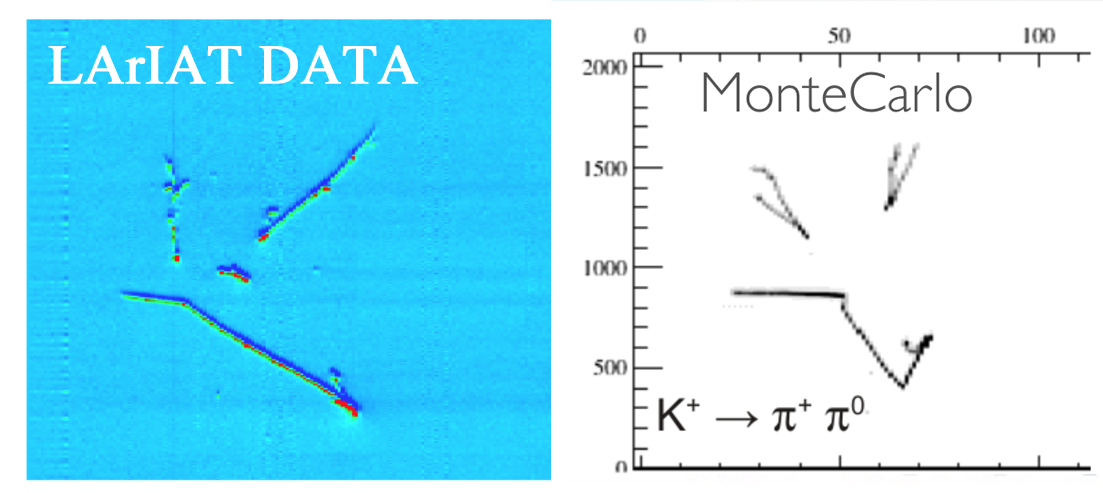
\includegraphics[width=6in]{images/Lariat/KDataMC}
\caption{Direct comparson between a kaon event in LArIAT Run I data and in LArIAT MC. }
\label{fig:MCdata}
\end{figure}


\begin{figure}[h!]
\centering
\begin{minipage}{0.45\textwidth}
\centering
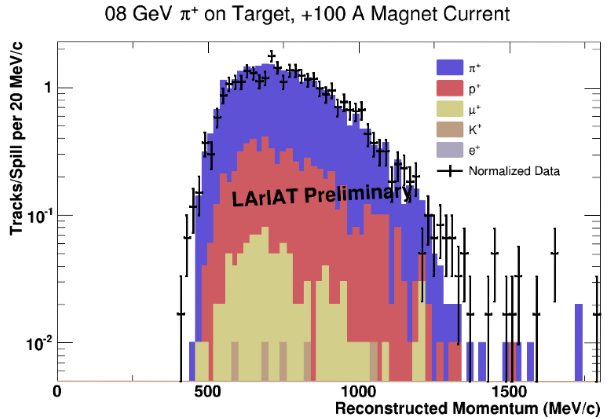
\includegraphics[width=3.5in]{images/Lariat/Beam}
\caption{Particle spectrum at the TPC produced with the LArIAT 8 GeV tertiary beam.}
\label{fig:BeamComp}
\end{minipage}\hfill
\centering
\begin{minipage}{0.45\textwidth}
\centering
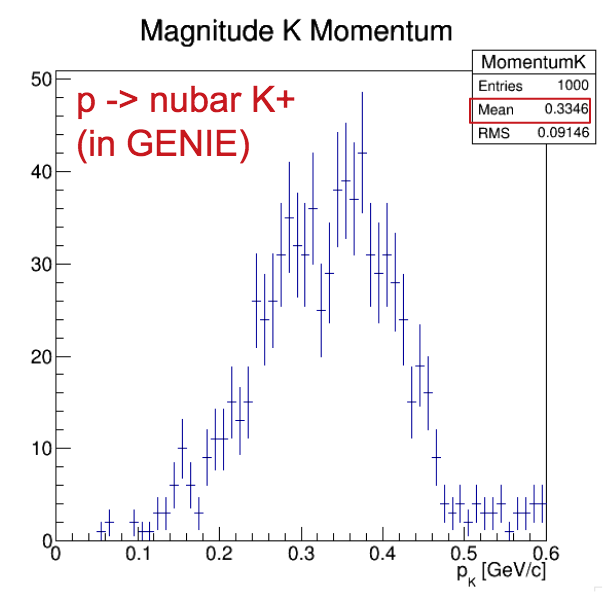
\includegraphics[width=3in]{images/Lariat/KaonGenie}
\caption{Momentum distribution for the kaon in the $p \rightarrow K^{+} \bar\nu$ mode proton decay as simulated by GENIE.}
\label{fig:KGenie}
\end{minipage}
\end{figure}





\begin{center}
\begin{table}[b]
	\begin{center}
	%\resizebox{0.95\textwidth}{!}{%
	\begin{tabular}{|c|c|c|}
	\multicolumn{3}{c}{\textbf{Summary of Data Samples}} \\
	\hline \hline
	 Run Period & Data Set Definition & Samweb Meaning \\
%	\hline
%	 &  & \verb!defname: TPC_voltages_nominal! \\
%	\hline
%	 &  & \verb!TPC_MaxGainAndFilter! \\
%	\hline
%	Run-I & \verb!Lovely1_Neg_RunI_elenag_v02! & \verb!TPC_nominal_read_out_and_timing!  \\
%	\hline
%	 & & \verb!BothTOF_OnAndReadOut!  \\
%	\hline
%	 & & \verb!AllMWPC_OnAndReadOut!  \\
%	 \hline
%	 & & \verb!lariat_mid_f_mc7anb < 0! \\
%	\hline
%	\line
%	 & & \verb!run_number >= 8000 and run_number <= 10226! \\
     \hline	
	&  & \verb!defname: TPC_voltages_nominal! \\
	\hline
	 &  & \verb!TPC_MaxGainAndFilter! \\
	\hline
	Run-II & \verb!Lovely1_Pos_RunII_elenag_v04! & \verb!TPC_nominal_read_out_and_timing!  \\
	\hline
	 & & \verb!BothTOF_OnAndReadOut!  \\
	\hline
	 & & \verb!AllMWPC_OnAndReadOut!  \\
	 \hline
	 & & \verb!lariat_mid_f_mc7anb > 0! \\
	 	 \hline
	 & & \verb!create_date < '2017-06-02'! \\

	 \hline
	\end{tabular}%}
	\caption{Summary of the data sample used for this analysis. }
	\label{tab:datasamples}
	\end{center}
\end{table}
\end{center}

The Run-II data use the definitions \href{https://redmine.fnal.gov/redmine/projects/lardbt/wiki/Recommended_SAM_Datasets}{oulined on this Wiki page} and summarized in Table \ref{tab:datasamples}.


The relevant \texttt{samweb} definitions listed in Table \ref{tab:datasamples} which require some explaining are defined as:

\begin{itemize}
\item \textbf{TPC Voltages Nominal}: Requires the cathode to be at greater than 23 kV, the collection plane wires voltage to be between 320 and 350 V, the induction plane voltage to be between -10 and -20 V, and the shield plane voltage to be greater than -310 V

\item \textbf{TPC MaxGainAndFilter}: Requires the ASIC configuration to be set as ``3'' for both the filter and the gain setting

\item \textbf{TPC Nominal Read Out and Timing}: Requires the readout of the TPC was enabled, the recorded number of time ticks is 3072, and the delay of 36900 was set on the v1495 (trigger card).
\item \textbf{lariat\_mid\_f\_mc7anb \textgreater 0} : Requires the polarity of the magnets to be positive
\item \textbf{create\_date \textless  2017-06-02}: Avoids the introduction of run 3 data and newly sliced data
\end{itemize}


It is important to provide a break down of the beam conditions for the period of data taking because the beam composition, hence the kaon content, varies according to the energy of the secondary beam and the strength of the magnetic field. Table \ref{tab:beamConditions} shows a break down of the beam conditions for the beam data selected by  \verb!Lovely1_Pos_RunII_elenag_v04! and the events that pass the beam line  selection.


\begin{table}[]
\centering
\caption{Break down of beam conditions for Run-II positive polarity data. $I$ is the value of the current in the magnets and $E$ is the energy of the secondary beam.  }
\label{tab:beamConditions}
\begin{tabular}{l|l|l|l|l|}
\cline{2-5}
                                       & \multicolumn{2}{l|}{Lovely1\_Pos\_RunII\_elenag\_v04} & \multicolumn{2}{l|}{Beamline Kaon candidate sample} \\ \cline{2-5} 
                                       & Run \% & Event \% & Run \% & Event \% \\ \hline
\multicolumn{1}{|l|}{I = + 100 A, E = 64 GeV}   &   61.8          &        75.0   & 75.1  &  90.35   \\ \hline
\multicolumn{1}{|l|}{I =   + 60 A, E = 64 GeV}   &    30.1         &         23.8  & 24.9  &   9.65     \\ \hline
\multicolumn{1}{|l|}{Info not available}              &      8.1         &           1.2   &    0.0 &       0.0               \\ \hline
\end{tabular}
\end{table}



%%%%%%%%%%%%%%%%%%%%%%%%%%%%%%%%%%%%%%%%%%%%%%%%%%%%%%%%%%%%
\subsection{Monte Carlo Samples}\label{sec:MCSamples}
For the simulation of the tertiary beam, we use a combination of two MC generators: the G4Beamline Monte Carlo and the Data Driven single particle Monte Carlo (DDMC).   We use the G4Beamline MC to calculate the particle composition of the beam just before the cryostat. In order to simulate the beam line particles after Wire-Chamber 4, we use the DDMC. 

\subsubsection{G4Beamline }\label{sec:G4Beamline}
At the moment of this writing,  G4Beamline simulates transportation of particles through the beam line from the LArIAT target until ``Big Disk'', a fictional, void detector located just before the cryostat. The responses of  the beam line detectors are not simulated. 

The two beam conditions relevant for this analysis are simulated: secondary beam energy of 64 GeV, positive polarity magnet with current of 100 A and 60 A. Figure \ref{fig:beamspectrum} shows the tertiary beam spectra for the 64 GeV and 100 A condition on the left and for the 64 GeV and 60 A condition on the right.
In Table \ref{tab:beamcomp2}, the beam composition is given in terms of percentage of different particle species per spill for positive polarity. The values reported are the weighted average on the two beam conditions considered. The weights are calculated according to the fourth column of Table \ref{tab:beamConditions}. 

\begin{table}[ht!]
\centering
\begin{tabular}{|l|l|l|l|l|l|l|}
\hline
                   & $\pi^+$ & $e^+$ & $\gamma$ & $\mu^+$ & $K^+$ & p \\ \hline
Beam Composition (\%) &    42.8     &  30.1     &    8.6      &    2.1     &    0.057    &    16.2            \\ \hline
\end{tabular}
\caption{Beam Composition - Positive polarity configuration (from MC)}
\label{tab:beamcomp2}
\end{table}



\begin{figure}[htb]
\begin{center}

\includegraphics[scale=0.05]{images/dummy.png}
\end{center}
\caption{G4Beamline tertiary beam  predicted spectra for positive 100 Amp, 64 GeV target energy with data overlaid (left). G4Beamline tertiary beam  predicted spectra for positive 60 Amp, 64 GeV target energy with data overlaid (right).}
\label{fig:beamspectrum}
\end{figure}



\subsubsection{Data Driven Single Particle MC (DDMC) }\label{sec:DDMCSamples}
%%%%%%%%%%%%%%%%%%%%%%%%%%%%%%%%%%%%%%%%%%%%%%%%%%%%%%%%%%%%
The DDMC uses the data momentum and position at wire chamber 4 to derive its initial conditions. The details of these samples and where they can be found are given in \href{https://docs.google.com/spreadsheets/d/1_0kNCKBIIx53f6vopqN2OijtcTICHD9rDvN_YKGH2mI/edit?usp=sharing}{this data production spreadsheet}.
More details of how the Monte Carlo used is generated are given in \href{https://lartpc-docdb.fnal.gov:441/cgi-bin/ShowDocument?docid=2054}{docDB-2054} and  \href{https://lartpc-docdb.fnal.gov:441/cgi-bin/ShowDocument?docid=2056}{dobDB-2056}, a summary of which is presented here. 

The Data Driven Monte Carlo (DDMC) uses data quantities for a sample of Wire-Chamber tracks to derive the momentum ($P_x, P_y, P_z$) and position at WC4 $X, Y$ distributions that are seen during a particular running period and/or running condition. Using those data derived distributions, it then launches single particle MC from $z = -100$~cm (the location of the fourth wire chamber) with these distributions as a template. An illustration of this procedure is shown in Figure \ref{fig:DDMC} with the results of the DDMC generation compared to a sample of wire chamber track data. Using this technique ensures the MC and data have very similar momentum, position and angular distributions at Wire-Chamber 4 and allow us to calibrate the energy loss upstream of the TPC as precisely as possible. The DDMC is a single particle Monte Carlo: the beam pile-up is not simulated.

\begin{figure}[htb]
\centering
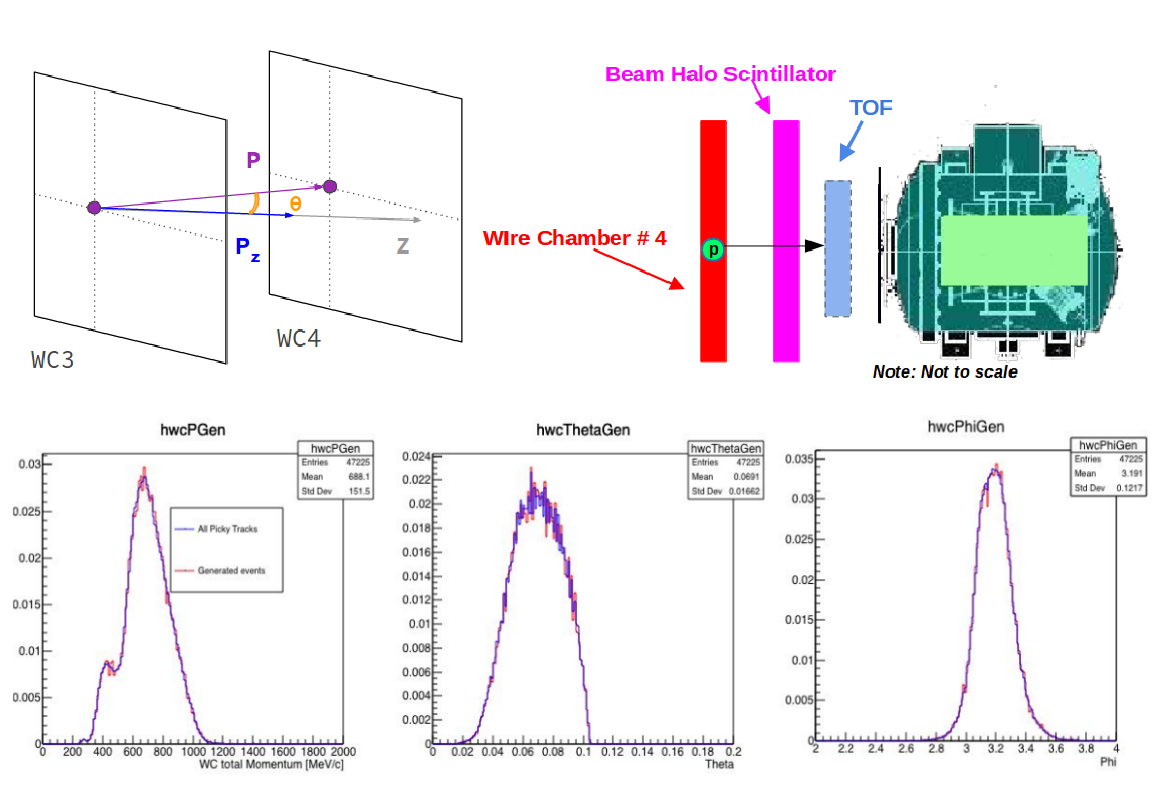
\includegraphics[width=0.70\textwidth]{images/DDMC.png}
\caption{Illustration of the technique where the wire chamber track initial angular and momentum distributions are used to generate the single particle MC.}
\label{fig:DDMC}
\end{figure}

Table \ref{tab:MCSampleGen} lists the various MC samples that were generated for this analysis. 

\begin{table}[htb]
	\begin{center}
	\resizebox{0.95\textwidth}{!}{%
	\begin{tabular}{|c|c|c|}
	\hline
	  \textbf{DDMC Sample} & Original Data Distribution & Number of Events Generated  \\
	  	\hline
	Run-II $\pi^{+}$ & $\pi, \mu, e$ Mass Filter / Picky WC-Track & \\
	Run-II $\mu^{+}$ & $\pi, \mu, e$ Mass Filter / Picky WC-Track &  \\
	Run-II $e^{+}$ & $\pi, \mu, e$ Mass Filter / Picky WC-Track & \\
	Run-II $K^{+}$ & $K^{+}$ Mass Filter / Picky WC-Track & \\
	Run-II $p$ & $p$ Mass Filter / Picky WC-Track & \\
	\hline
	\end{tabular}}
	\caption{Summary of MC generated for the analysis.} \label{tab:MCSampleGen}
	\end{center}
\end{table}

\textcolor{red}{CHECK WITH THE BEAMLINE MC IF WE REALLY NEED THIS}
In addition to this sample of DDMC, a sample of photons is also generated since as is shown in Table \ref{tab:beamcomp1} a small but non-negligible portion of the beam will have photons entering the TPC. This sample is generated with a flat momentum spectrum between 0 MeV and 2000 MeV with a Gaussian angular distribution of $\pm$5 degrees about the beam direction. The photon momentum spectrum is then re-weighted by the momentum spectrum of the corresponding run period it is being simulated for. This approximation allows us to estimate the contamination due to photons from MC with a reasonable assumption of their spectrum.






%%%%%%%%%%%%%%%%%%%%%%%%%%%%%%%%%
%% SECTION 4
%%%%%%%%%%%%%%%%%%%%%%%%%%%%%%%%%
%%\section{\textcolor{blue}{R\&D Strategy}}
%\include{section4}
%\input{section4}

%%%%%%%%%%%%%%%%%%%%%%%%%%%%%%%%%
%% SECTION 5
%%%%%%%%%%%%%%%%%%%%%%%%%%%%%%%%%
%\include{section4}
%\section{Inclusive $\pi^{-}$-Argon Cross-Section} \label{sec:CrossSection}
Finally, we come to the inclusive $\pi^{-}$-Argon cross-section result for the data and MC samples defined previously.

The incident kinetic energy is defined as
\begin{equation}
KE_{Incident} = \sqrt{P_{WCtrk}^2 + m_{\pi}^2} - m_{\pi}^2 - E_{Loss} - (\Sigma dE/dX_{i} \times Pitch)
\end{equation}
up to the point of where the track either has an interaction and thus reaches the end of track in the volume or exits out the back. The distribution is shown in Figure \ref{fig:IncidentEnergy}.

\begin{figure}[h!]
\centering
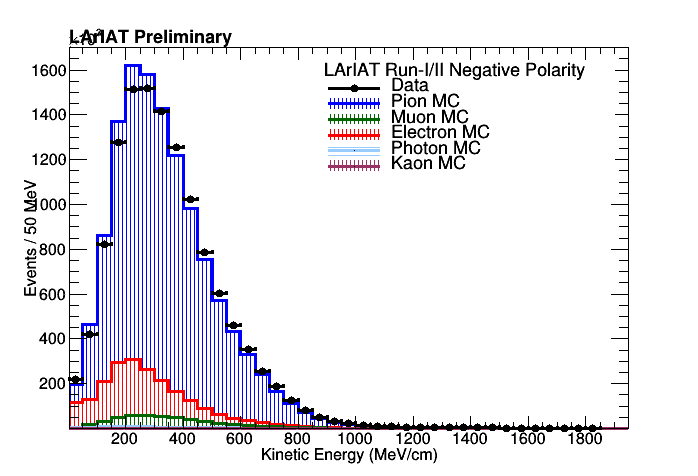
\includegraphics[scale=0.30]{./images/IncidentKE.png}
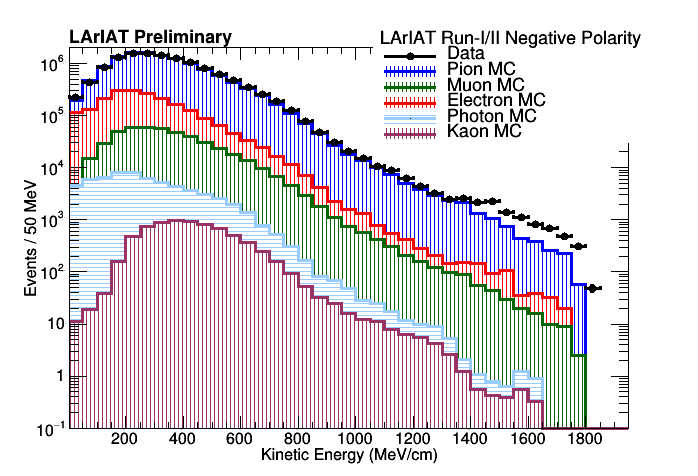
\includegraphics[scale=0.30]{./images/IncidentKELog.png}
\caption{Incident kinetic energy distribution. (Note: the distribution on the left is linear scale in the y-axis, and the distribution on the right is log scale on the y-axis).}
\label{fig:IncidentEnergy}
\end{figure}

Figure \ref{fig:InteractingEnergy} shows the kinetic energy distribution for the interaction point. Tracks which exit out of the active volume of the TPC without having an interaction are excluded from this plot.

\begin{figure}[h!]
\centering
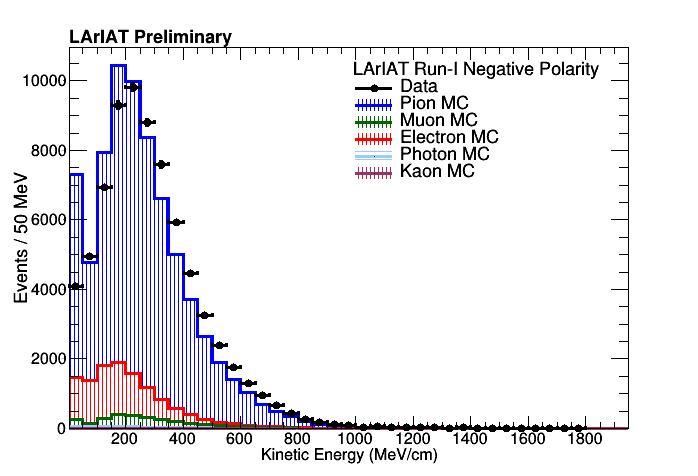
\includegraphics[scale=0.30]{./images/InteractingKE.png}
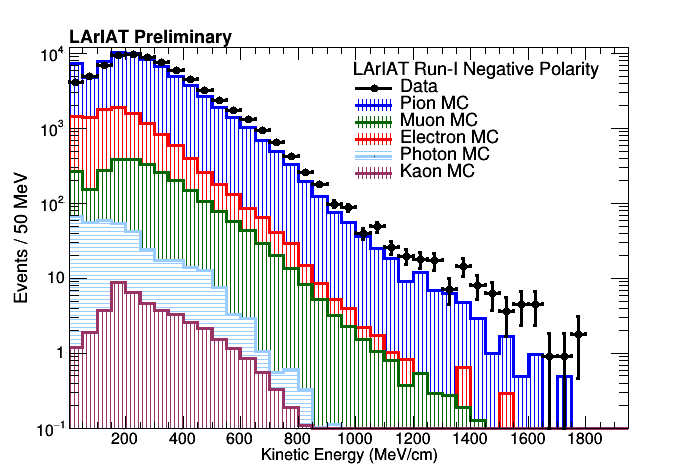
\includegraphics[scale=0.30]{./images/InteractingKELog.png}
\caption{Interacting kinetic energy distribution. (Note: the distribution on the left is linear scale in the y-axis, and the distribution on the right is log scale on the y-axis).}
\label{fig:InteractingEnergy}
\end{figure}

We calculate the cross-section according to the method described in Section \ref{sec:ThinSlice}, correcting for the crossing muon contamination (estimated at 9$\%$), as explained in Appendix \ref{appendix:CrossingMuon}. Figure \ref{fig:RawCrossSection} shows the full range of the computed cross-section including negative kinetic energy bins (between -100 MeV and 0 MeV). There are a few features worth noting about this plot.

\begin{itemize}
\item \textbf{Negative Energy Bins}: The data and the MC don't agree at all in the negative energy bins.

\item \textbf{0~MeV$<$KE$<$50~MeV}: This is the only physical bin in which the data and MC disagree strongly. As outlined in Section \ref{sec:MCReduction}, this bin is expected to be dominated by pion capture-at-rest and should be excluded from the interaction cross-section. This may suggest that the rate at which these events occur is different between data and MC and, while interesting, is beyond the scope of this analysis.

\item \textbf{KE $>$ 50~MeV}: There is generally good agreement above 50~MeV between data and MC.

\end{itemize}

\begin{figure}[h!]
\centering
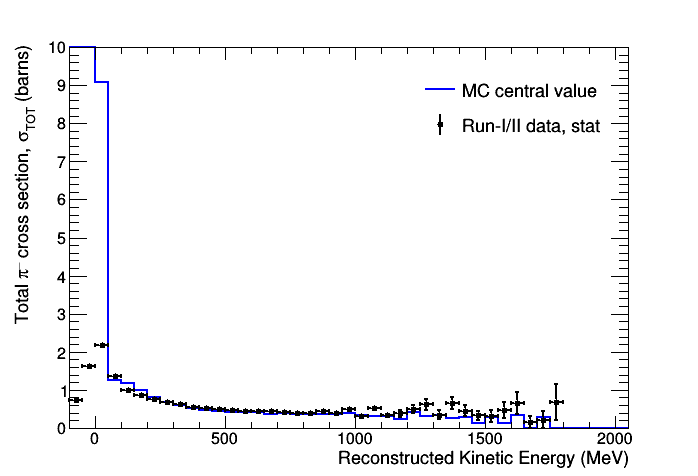
\includegraphics[scale=0.30]{./images/CombinedNegPol_xsec_MC_noband_fineBin.png}
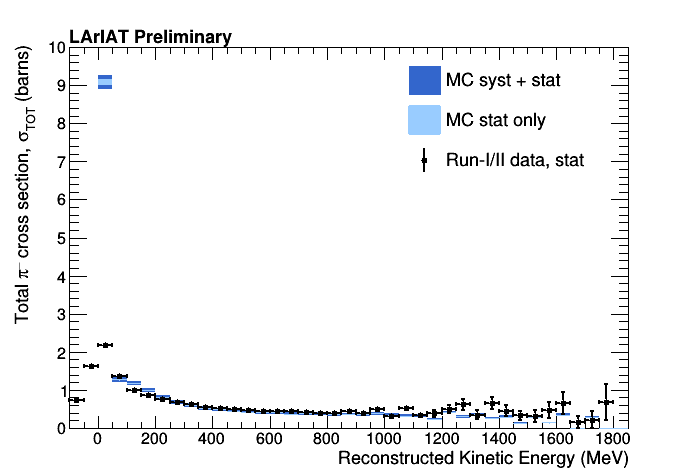
\includegraphics[scale=0.30]{./images/CombinedNegPol_xsec_MCband_opt2FineBin.png}
\caption{Total cross-section computed across the full kinetic energy range (including negative KE bins). The LHS shows the data (black) and the MC central value (blue). The RHS shows the same but with systematic errors associated. }
\label{fig:RawCrossSection}
\end{figure}

Figure \ref{fig:ProperBinCrossSection} shows the inclusive cross-section zoomed in between 50~MeV$<$KE$<$1800 MeV.

\begin{figure}[h!]
\centering
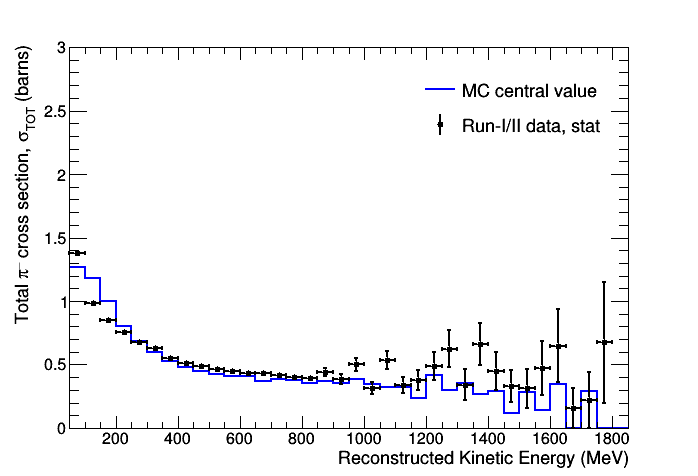
\includegraphics[scale=0.30]{./images/CombinedNegPol_xsec_MC_noband_fineBinProper.png}
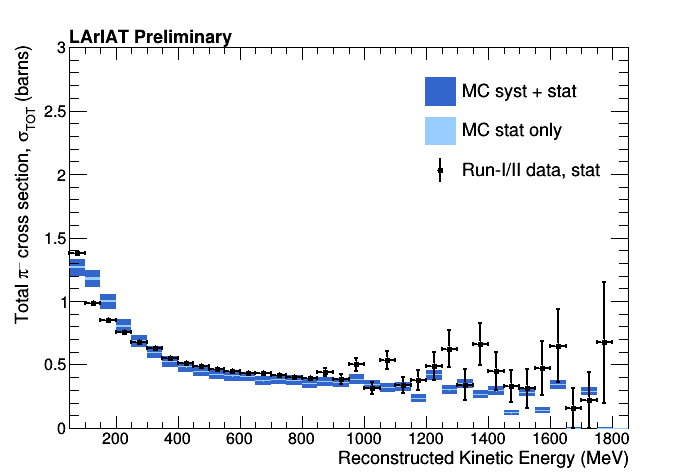
\includegraphics[scale=0.30]{./images/CombinedNegPol_xsec_MCband_opt1FineBinProper.png}
\caption{Total cross-section in the region between 50~MeV$<$KE$<$1800 MeV. The LHS shows the data (black) and the MC central value (blue). The RHS shows the same but with systematic errors associated. }
\label{fig:ProperBinCrossSection}
\end{figure}

Figure \ref{fig:VariableBinCrossSection} shows the final result for the cross-section. In the region between 300~MeV and 1200~MeV the data is 6-8$\%$ higher than the Monte Carlo prediction, but within the systematic uncertainty of the measurement. The region below 300~MeV is data is low compared to the MC (with the exception of the lowest energy bin).


\begin{figure}[h!]
\centering
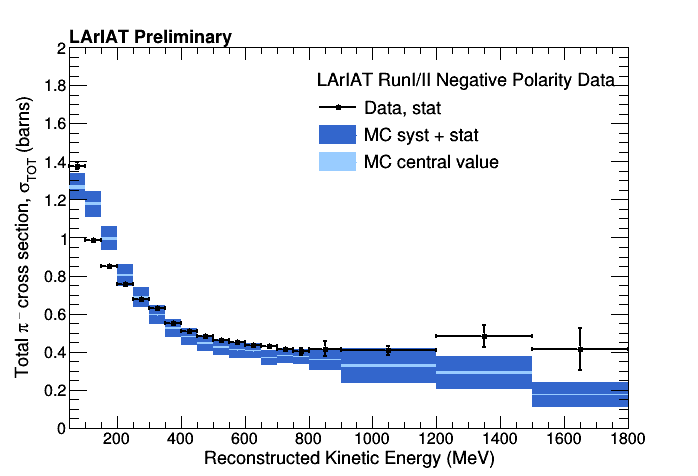
\includegraphics[scale=0.60]{./images/TotalCrossSection.png}
\caption{Total cross-section in the region between 50~MeV$<$KE$<$1800 MeV. }
\label{fig:VariableBinCrossSection}
\end{figure}

\clearpage


\newpage

\newpage
\clearpage
\appendix
%\section{Appendix 1: Crossing Muons} \label{appendix:CrossingMuon}
Particles with energies higher than $\approx$ 150 MeV can cross the TPC volume and exit the TPC without experiencing an interaction. We define as “crossing” each particle that exits the TPC fiducial boundaries.\\
These particles will then contribute only in filling the $N_{incident}$ histogram for each point of their track, meaning that for the energies related to the track points they are more likely to survive than to interact with Ar nuclei.\\

The percentage of crossing tracks from the Closed Box data sample are reported in Tab.\ref{tabellaCrossing}. In Fig.\ref{CrossingOBKinEn} the Incident and Final kinetic energy of crossing tracks in the Open Box sample is reported.
\begin{table}[ht!]
\centering
\begin{tabular}{|c|c|}
\hline
\textbf{Event Sample} & \textbf{Number of Events} \\ 
\hline \hline
Run I Negative Polarity Data Sample                                                                          & 486753           \\
\hline
After all selection cuts                                                                      & 2404             \\
\hline
Crossing tracks                                                                               & 858              \\
\hline
\% Crossing tracks over events that pass all cuts & 35.7 \%\\          
\hline
\end{tabular}
\caption{Crossing tracks after all the selection cuts for a subsample of Run-I data.} 
\label{tabellaCrossing}
\end{table}

\begin{figure}[h!]
\centering
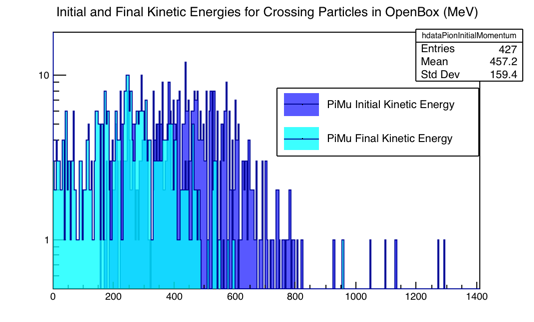
\includegraphics[scale=0.45]{./images/OBparticles_crossingKinEn.png}
\caption{Initial and Final kinetic energy spectra for Crossing tracks ifor a subsample of Run-I data.}
\label{CrossingOBKinEn}
\end{figure}

We know the particles from the beamline which can exit the TPC boundaries will be mainly pions and muons. It is then natural to evaluate the percentage of contamination by muons in our "crossing particles" data sample. Since crossing muon tracks will be taken into account when filling the $N_{incident}$ histogram for the Pion cross section evaluation. The {\textbf{crossing muon contamination}} in $N_{incident}$ will then affect our measurement.

We agreed to provide an estimate for the contribution of "crossing muon" events via Monte Carlo simulation. We will then apply this "crossing muon contamination" correction on the $N_{incident}$ histogram made from the data sample.\\
We made a study of crossing track events from the MC sample of pions and muons (the incoming particles energy spectrum was re-weighted based on the beam profile). In Tab.\ref{tab:CrossingMC} we show the percentages of crossing pions and muons after our selection cuts, in case a fixed number of pions and muons are shot in our MC simulation. Muons are not strongly affected by our selection cuts and we see they're mostly crossing events (almost 76\% of the selected muon events are crossing tracks). Pion statistic is a bit more affected by our cuts than the muon's: 70.1\% of the pions that enter the TPC made it to pass all our selection cuts and only 32\% of them are crossing tracks, since most of them interact into the TPC volume.\\
% Considering crossing events, from Tab.\ref{tab:CrossingMC} we see:
% $$ \Big(\frac{\mu}{\pi}\Big)_{cross,cuts}^{MC, unweighted} \simeq 3 $$
% this is in case of same number of pions and muons shot via MC.
For our analysis, it is important to consider the relative fraction of pions and muons in the beam to get a proper estimate of the real crossing muon contamination of our sample. The muon to pion fraction from the beam composition is, for negative polarity runs (See Tab.\ref{tab:beamcomp1}): 
$$ \Big(\frac{\mu}{\pi}\Big)_{beam} \simeq 0.045 $$
%commented stuff - weird results - to be updated soon
Therefore if we weight by the beam composition the crossing muons to crossing pions ratio obtained before, we can get an average estimate over all energies for the $(\frac{\mu}{\pi})_{cross}$ we can expected in the Data:
$$ \Big(\frac{\mu}{\pi}\Big)_{cross,cuts}^{MC, weighted} \simeq  0.136 $$
The average MC estimate of the composition of Crossing Tracks sample is then: 88\% pions, 12\% muons.\\ 
% (on average - MC estimate): 
% Pi: 88 %
% Mu: 12 %
% (considering the beam composition and assuming ONLY Pi and Mu cross the TPC)

A more complete analysis has been made considering the crossing muon contamination in each energy bin of $N_{incident}$ histogram, as shown in Fig.\ref{CrossingMCNinc}, Fig.\ref{CrossingOBMuon} and Fig.\ref{CrossingFraction}. \\
The fraction of crossing muons in each energy bin of $N_{incident}$ histogram will actually make our denominator for cross section calculation higher then if we had only pions.
From the plot in Fig.\ref{CrossingFraction} we see the fractional contribution of crossing muons is quite flat, at least in the 50-650 MeV region.
We have decided to consider a uniform crossing muon contamination factor of the order of 10\% and to apply this correction in each energy bin of the $N_{incident}$ histogram made from our Data sample. This results in a 9\% reduction of the content of each energy bin. We will also assume a 20\% uncertainty on our estimate of the crossing muon contamination factor in $N_{incident}$, that will reflect in a $\approx$ 3\% systematic on the cross section measurement for each energy bin.

$$ N_{incident}^{data} \longrightarrow N_{incident}^{data, \mu corr} \text{ applied 9\% crossing $\mu$ contamination correction}$$
$$\sigma \approx \frac{N_{incident}^{data}}{N_{incident}^{data, \mu corr}} \text{ , } \Big(\frac{\Delta\sigma}{\sigma}\Big)_{sys}^{\mu corr} \simeq 3 \% $$ 


\begin{table}[ht!]
\centering
\begin{tabular}{|l|l|l|}
\hline
\textbf{Event Sample}                                                                                 & {\textbf{Pions}} & {\textbf{Muons}} \\ \hline \hline
MC sample                                                                                     & 118800 & 79200 \\ \hline
MC sample - particles that enter the TPC                                                      & 80603 & 76328 \\ \hline
After all selection cuts                                                                      & 56462 & 63146 \\ \hline
Crossing tracks                                                                               & 26035  & 58261 \\ \hline
\% Crossing tracks  & 32.3 \% & 76.3 \% \\ \hline
\end{tabular}
\caption{Crossing tracks after all the selection cuts for pions and muons (from MC).}
\label{tab:CrossingMC}
\end{table}


% \begin{figure}[h!]
% \begin{minipage}{0.5\textwidth}
% 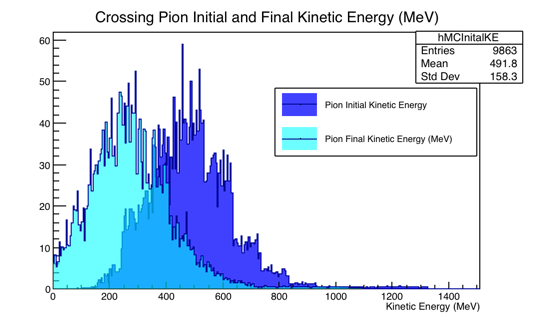
\includegraphics[width=\textwidth]{PionCrossingKinEn.png}
% \end{minipage}
% \begin{minipage}{0.5\textwidth}
% 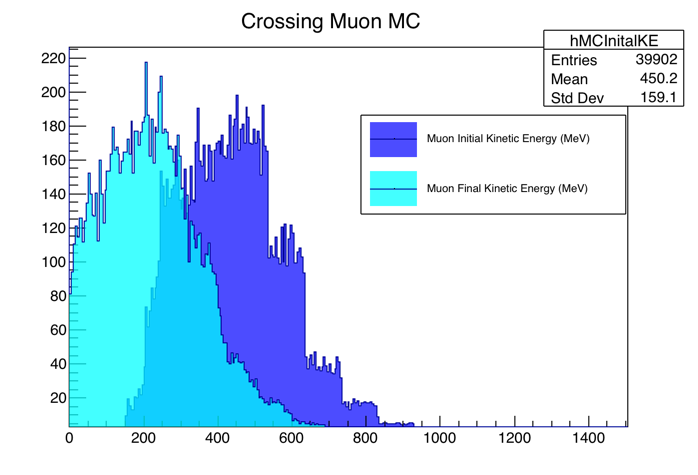
\includegraphics[width=\textwidth]{CrossMuKinEn.png}
% \end{minipage}
% \caption{Initial and Final kinetic energy spectra for Crossing Pion and Muon tracks from MC Sample.}
% \label{CrossingMCPionKinEn}
% \end{figure}

% \begin{figure}[h!]
% \centering
% 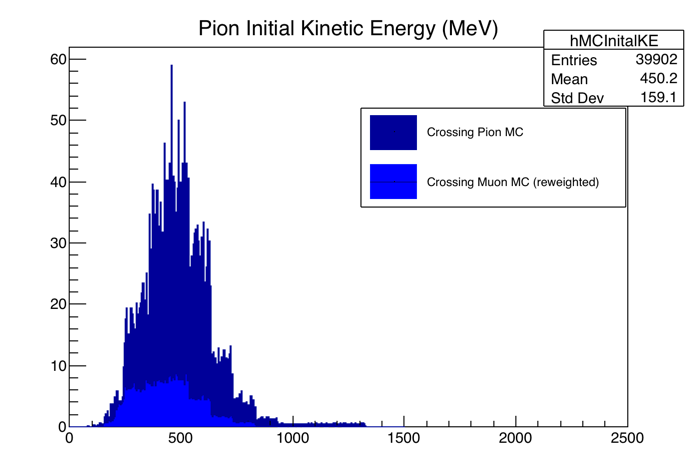
\includegraphics[scale=0.4]{CrossMuPiKinEn.png}
% \caption{Initial kinetic energy spectra for Crossing Pion and Muon tracks from MC Sample weighted by beam composition.}
% \end{figure}

\begin{figure}[h!]
\begin{minipage}{0.5\textwidth}
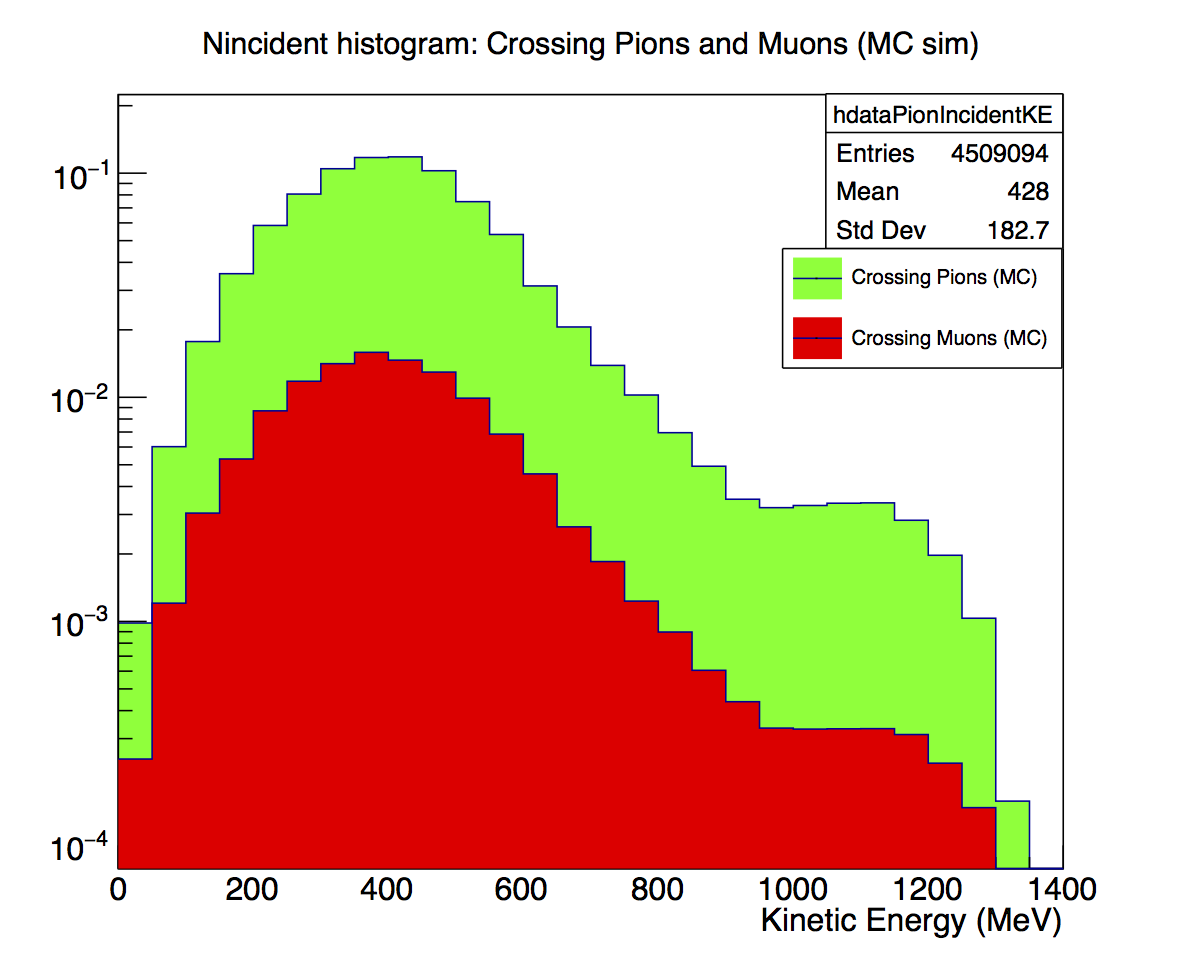
\includegraphics[width=\textwidth]{./images/CrossingPiMu.png}
\end{minipage}
\begin{minipage}{0.5\textwidth}
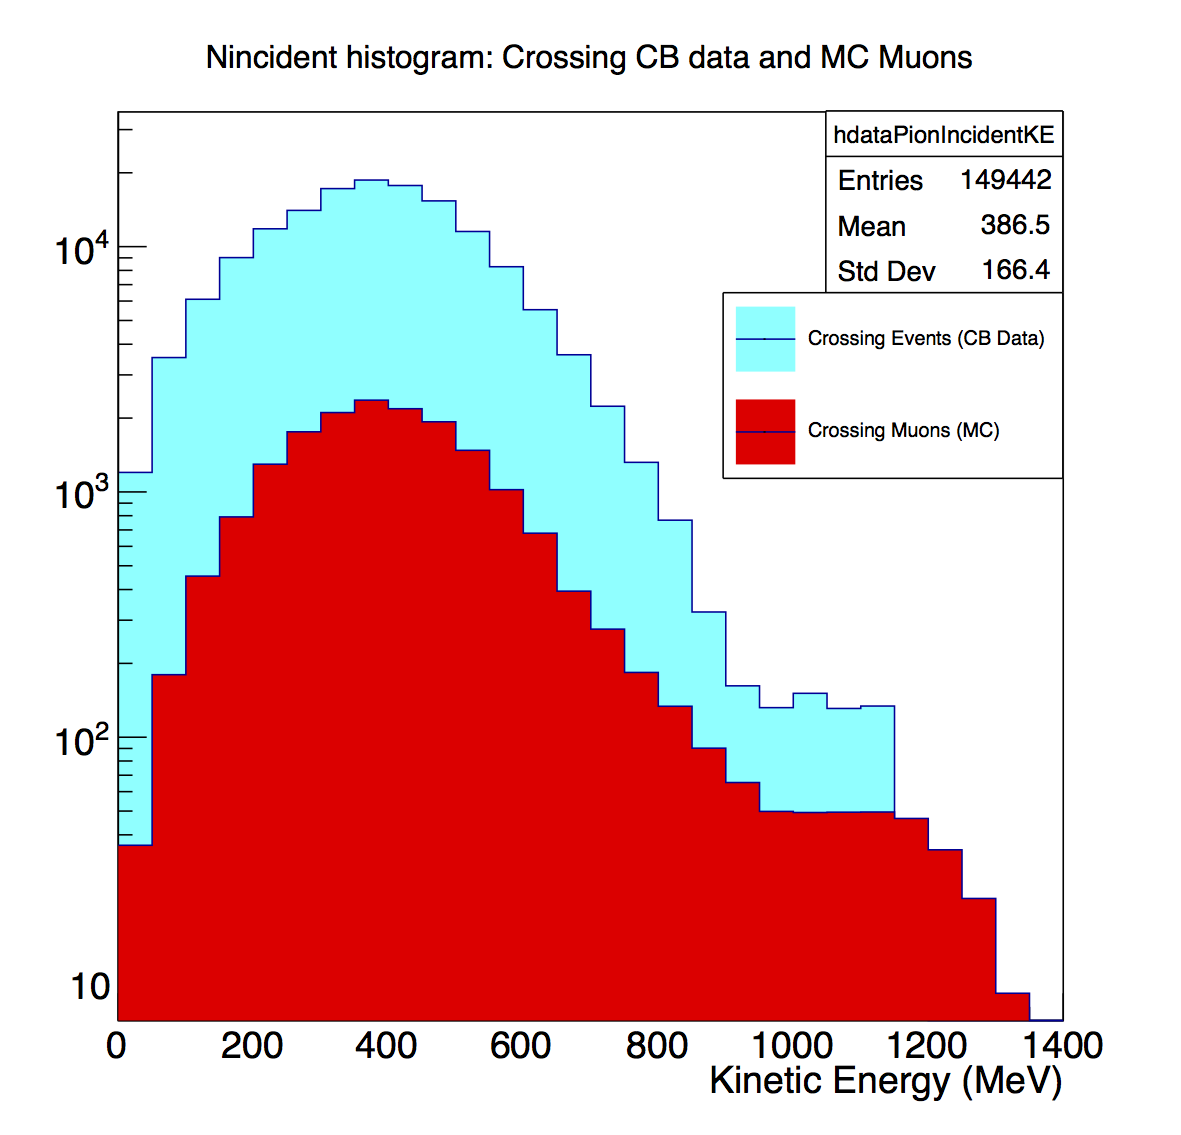
\includegraphics[width=\textwidth]{./images/CrossingCBandMuMC.png}
\end{minipage}
\caption{$N_{incident}$ histogram for Crossing Pion and Muon tracks from MC Sample weighted by muon to pion ratio from the beam composition. (The histogram is normalized to the sum of crossing Muons and crossing Pions statistic - the total of crossing events).[left] $N_{incident}$ histogram for Run I Neg.Pol. Data sample (CB) Crossing Events and for Crossing Muon tracks from MC Sample.[right]}
\label{CrossingMCNinc}
\end{figure}

\begin{figure}[h!]
\centering
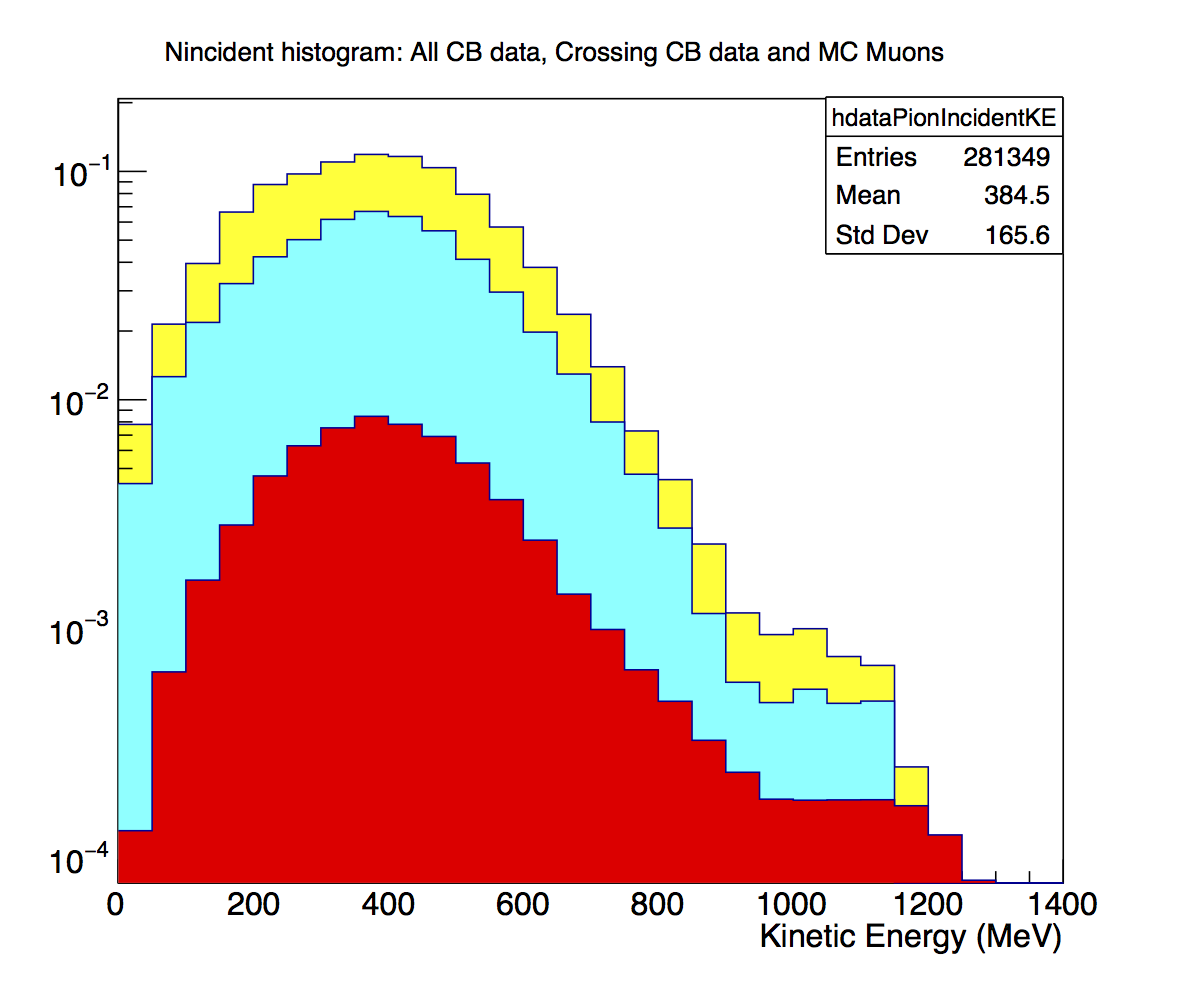
\includegraphics[scale=0.5]{./images/CBAllandCross_CrossMuMC.png}
\caption{$N_{incident}$ histogram for for a subsample of Run-I data (All [yellow] and only crossing [cyan]) and for Crossing Muon tracks from MC Sample [red]. (The histograms are normalized to the the data statistic in $N_{incident}$.)}
\label{CrossingOBMuon}
\end{figure}

\begin{figure}[h!]
\centering
%\includegraphics[scale=0.4]{./images/CrossMu_FractionOK.pdf}
\caption{Crossing Muon fraction on for a subsample of Run-I data in $N_{incident}$ histogram. }
\label{CrossingFraction}
\end{figure}

\newpage
\clearpage
%\section{Appendix 2: Energy subtraction due to upstream material}\label{appendix:EnergyCorrections}
%%%%%%%%%%%%%%%%%%%%%%%%%%%%%%%%%%%%%%%%%%%%%%%%%%%%%%%%%%%%%%%%

Figure \ref{fig:EndPointPionMCInBeamLine} shows the end point position for the single particle $\pi$ Monte Carlo launched from $z=-100$~cm. This ``x-ray'' plot demonstrates the upstream material that is present in the LArIAT simulation of the beamline. While a large number of the simulated particles manage to enter the TPC, they will interact with the material and thus lose energy prior to being measured in the TPC.

\begin{figure}[h!]
\centering
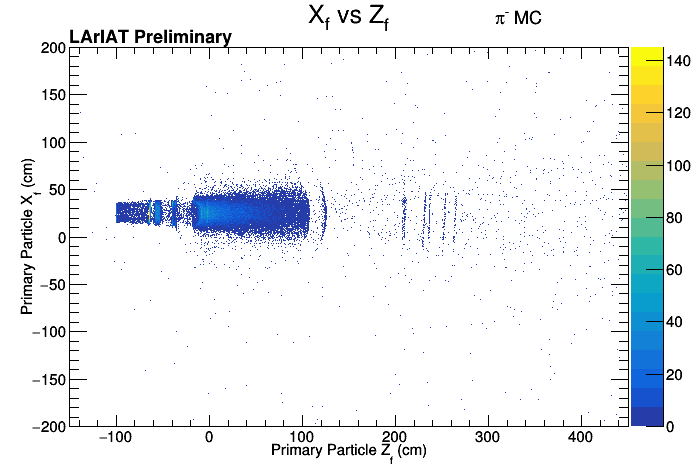
\includegraphics[scale=0.45]{./images/UnweightedXfvsZf.png}
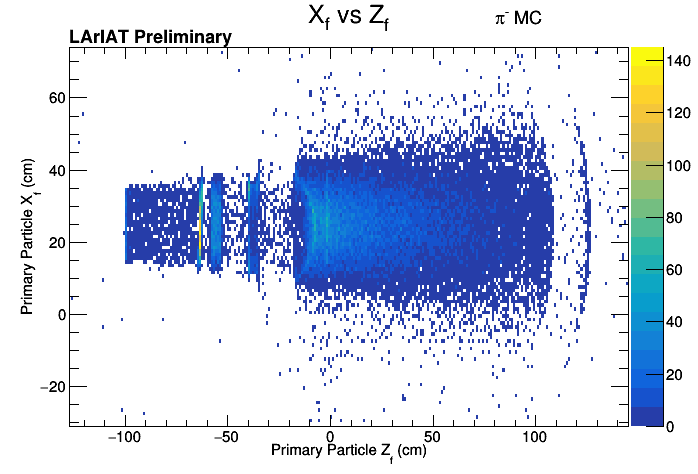
\includegraphics[scale=0.45]{./images/UnweightedXfvsZfupstreamzoom.png}
\caption{End point position for a sample of single particle $\pi^{-}$ MC showing the simulated upstream material and the interaction the pions can have with it.}
\label{fig:EndPointPionMCInBeamLine}
\end{figure}

This process obviously occurs in the data as well, and needs to be accounted for when taking the momentum of the particle measured from the wire chambers and extrapolating this to the TPC. In order to assess how much energy is loss for a pion traversing the material between Wire Chamber four and the front face of the active volume of the TPC, we take the $\pi$ MC and add up all the energy loss between the generation point ($z = -100$~cm) and the TPC ($z=0$~cm). Figure \ref{fig:EnergyLoss} shows the sum of all the energy loss for each pion prior to the particle entering the TPC. Any pion which does not have a trajectory which intercepts the TPC (e.g. interacts strongly in the upstream material) is excluded from this plot.

\begin{figure}[h!]
\centering
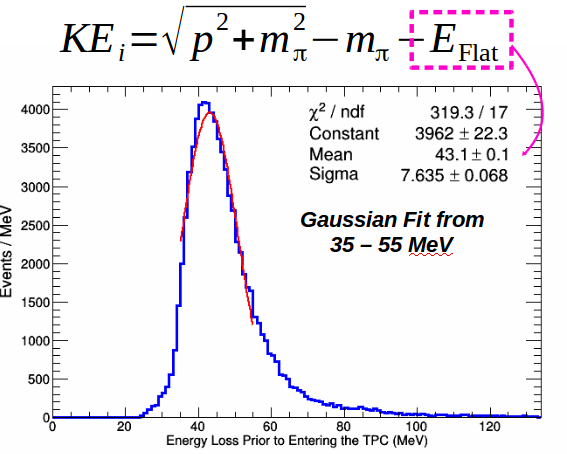
\includegraphics[scale=0.45]{./images/Eloss.png}
\caption{Energy loss from pions interacting in the simulated upstream material.}
\label{fig:EnergyLoss}
\end{figure}

Fitting the peak with a Gaussian, the most mean value is given as 40~MeV. The correction due to the energy loss from the upstream material is applied when calculating the initial kinetic energy as the term $E_{Flat}$

\newpage
%%%%%%%%%%%%%%%%%%%%%%%%%%%%%%%%%
%%  BIBLIOGRAPHY	
%%%%%%%%%%%%%%%%%%%%%%%%%%%%%%%%%
%\begin{thebibliography}{99}
\footnotesize

%1
\bibitem{PDG}
PASSAGE OF PARTICLES THROUGH MATTER, . Nakamuraet al.(PDG), JP G37, 075021 (2010) and 2011 partial update for the 2012 edition \url{http://pdg.lbl.gov/2011/reviews/rpp2011-rev-passage-particles-matter.pdf}.

%2
\bibitem{PDG-Argon}
PDG Tables for Liquid Argon \url{http://pdg.lbl.gov/2017/AtomicNuclearProperties/MUE/muE_liquid_argon.txt}. 

\bibitem{WCTrackReco}
Wire Chamber Track Reconstruction, LArIAT DocDB 1771 \url{https://lartpc-docdb.fnal.gov:441/cgi-bin/ShowDocument?docid=1771}

\end{thebibliography}
\textbf{}
\bibliographystyle{plain}
\bibliography{bib}

%\begin{thebibliography}{99}
\footnotesize

%1
\bibitem{PDG}
PASSAGE OF PARTICLES THROUGH MATTER, . Nakamuraet al.(PDG), JP G37, 075021 (2010) and 2011 partial update for the 2012 edition \url{http://pdg.lbl.gov/2011/reviews/rpp2011-rev-passage-particles-matter.pdf}.

%2
\bibitem{PDG-Argon}
PDG Tables for Liquid Argon \url{http://pdg.lbl.gov/2017/AtomicNuclearProperties/MUE/muE_liquid_argon.txt}. 

\bibitem{WCTrackReco}
Wire Chamber Track Reconstruction, LArIAT DocDB 1771 \url{https://lartpc-docdb.fnal.gov:441/cgi-bin/ShowDocument?docid=1771}

\end{thebibliography}
\textbf{}


\end{document}